\documentclass[]{tufte-book}

% ams
\usepackage{amssymb,amsmath}

\usepackage{ifxetex,ifluatex}
\usepackage{fixltx2e} % provides \textsubscript
\ifnum 0\ifxetex 1\fi\ifluatex 1\fi=0 % if pdftex
  \usepackage[T1]{fontenc}
  \usepackage[utf8]{inputenc}
\else % if luatex or xelatex
  \makeatletter
  \@ifpackageloaded{fontspec}{}{\usepackage{fontspec}}
  \makeatother
  \defaultfontfeatures{Ligatures=TeX,Scale=MatchLowercase}
  \makeatletter
  \@ifpackageloaded{soul}{
     \renewcommand\allcapsspacing[1]{{\addfontfeature{LetterSpace=15}#1}}
     \renewcommand\smallcapsspacing[1]{{\addfontfeature{LetterSpace=10}#1}}
   }{}
  \makeatother
\fi

% graphix
\usepackage{graphicx}
\setkeys{Gin}{width=\linewidth,totalheight=\textheight,keepaspectratio}

% booktabs
\usepackage{booktabs}

% url
\usepackage{url}

% hyperref
\usepackage{hyperref}

% units.
\usepackage{units}


\setcounter{secnumdepth}{2}

% citations
\usepackage{natbib}
\bibliographystyle{apalike}

% pandoc syntax highlighting
\usepackage{color}
\usepackage{fancyvrb}
\newcommand{\VerbBar}{|}
\newcommand{\VERB}{\Verb[commandchars=\\\{\}]}
\DefineVerbatimEnvironment{Highlighting}{Verbatim}{commandchars=\\\{\}}
% Add ',fontsize=\small' for more characters per line
\usepackage{framed}
\definecolor{shadecolor}{RGB}{248,248,248}
\newenvironment{Shaded}{\begin{snugshade}}{\end{snugshade}}
\newcommand{\KeywordTok}[1]{\textcolor[rgb]{0.13,0.29,0.53}{\textbf{{#1}}}}
\newcommand{\DataTypeTok}[1]{\textcolor[rgb]{0.13,0.29,0.53}{{#1}}}
\newcommand{\DecValTok}[1]{\textcolor[rgb]{0.00,0.00,0.81}{{#1}}}
\newcommand{\BaseNTok}[1]{\textcolor[rgb]{0.00,0.00,0.81}{{#1}}}
\newcommand{\FloatTok}[1]{\textcolor[rgb]{0.00,0.00,0.81}{{#1}}}
\newcommand{\ConstantTok}[1]{\textcolor[rgb]{0.00,0.00,0.00}{{#1}}}
\newcommand{\CharTok}[1]{\textcolor[rgb]{0.31,0.60,0.02}{{#1}}}
\newcommand{\SpecialCharTok}[1]{\textcolor[rgb]{0.00,0.00,0.00}{{#1}}}
\newcommand{\StringTok}[1]{\textcolor[rgb]{0.31,0.60,0.02}{{#1}}}
\newcommand{\VerbatimStringTok}[1]{\textcolor[rgb]{0.31,0.60,0.02}{{#1}}}
\newcommand{\SpecialStringTok}[1]{\textcolor[rgb]{0.31,0.60,0.02}{{#1}}}
\newcommand{\ImportTok}[1]{{#1}}
\newcommand{\CommentTok}[1]{\textcolor[rgb]{0.56,0.35,0.01}{\textit{{#1}}}}
\newcommand{\DocumentationTok}[1]{\textcolor[rgb]{0.56,0.35,0.01}{\textbf{\textit{{#1}}}}}
\newcommand{\AnnotationTok}[1]{\textcolor[rgb]{0.56,0.35,0.01}{\textbf{\textit{{#1}}}}}
\newcommand{\CommentVarTok}[1]{\textcolor[rgb]{0.56,0.35,0.01}{\textbf{\textit{{#1}}}}}
\newcommand{\OtherTok}[1]{\textcolor[rgb]{0.56,0.35,0.01}{{#1}}}
\newcommand{\FunctionTok}[1]{\textcolor[rgb]{0.00,0.00,0.00}{{#1}}}
\newcommand{\VariableTok}[1]{\textcolor[rgb]{0.00,0.00,0.00}{{#1}}}
\newcommand{\ControlFlowTok}[1]{\textcolor[rgb]{0.13,0.29,0.53}{\textbf{{#1}}}}
\newcommand{\OperatorTok}[1]{\textcolor[rgb]{0.81,0.36,0.00}{\textbf{{#1}}}}
\newcommand{\BuiltInTok}[1]{{#1}}
\newcommand{\ExtensionTok}[1]{{#1}}
\newcommand{\PreprocessorTok}[1]{\textcolor[rgb]{0.56,0.35,0.01}{\textit{{#1}}}}
\newcommand{\AttributeTok}[1]{\textcolor[rgb]{0.77,0.63,0.00}{{#1}}}
\newcommand{\RegionMarkerTok}[1]{{#1}}
\newcommand{\InformationTok}[1]{\textcolor[rgb]{0.56,0.35,0.01}{\textbf{\textit{{#1}}}}}
\newcommand{\WarningTok}[1]{\textcolor[rgb]{0.56,0.35,0.01}{\textbf{\textit{{#1}}}}}
\newcommand{\AlertTok}[1]{\textcolor[rgb]{0.94,0.16,0.16}{{#1}}}
\newcommand{\ErrorTok}[1]{\textcolor[rgb]{0.64,0.00,0.00}{\textbf{{#1}}}}
\newcommand{\NormalTok}[1]{{#1}}

% longtable

% multiplecol
\usepackage{multicol}

% strikeout
\usepackage[normalem]{ulem}

% morefloats
\usepackage{morefloats}


% tightlist macro required by pandoc >= 1.14
\providecommand{\tightlist}{%
  \setlength{\itemsep}{0pt}\setlength{\parskip}{0pt}}

% title / author / date
\title{A MODERN DIVE into the Language of Science}
\author{Chester Ismay and Albert Y. Kim}
\date{2016-08-02}

\usepackage{booktabs}
\usepackage{longtable}
\usepackage{framed,color}
\definecolor{shadecolor}{RGB}{248,248,248}

\ifxetex
  \usepackage{letltxmacro}
  \setlength{\XeTeXLinkMargin}{1pt}
  \LetLtxMacro\SavedIncludeGraphics\includegraphics
  \def\includegraphics#1#{% #1 catches optional stuff (star/opt. arg.)
    \IncludeGraphicsAux{#1}%
  }%
  \newcommand*{\IncludeGraphicsAux}[2]{%
    \XeTeXLinkBox{%
      \SavedIncludeGraphics#1{#2}%
    }%
  }%
\fi

%% Need to clean up
\newenvironment{rmdblock}[1]
  {\begin{shaded*}
  \begin{itemize}
  \renewcommand{\labelitemi}{
    \raisebox{-.7\height}[0pt][0pt]{
  %    {\setkeys{Gin}{width=3em,keepaspectratio}\includegraphics{images/#1}}
    }
  }
  \item
  }
  {
  \end{itemize}
  \end{shaded*}
  }
%% Probably can be omitted
\newenvironment{rmdnote}
  {\begin{rmdblock}{note}}
  {\end{rmdblock}}
\newenvironment{rmdcaution}
  {\begin{rmdblock}{caution}}
  {\end{rmdblock}}
\newenvironment{rmdimportant}
  {\begin{rmdblock}{important}}
  {\end{rmdblock}}
\newenvironment{rmdtip}
  {\begin{rmdblock}{tip}}
  {\end{rmdblock}}
\newenvironment{rmdwarning}
  {\begin{rmdblock}{warning}}
  {\end{rmdblock}}
\newenvironment{learncheck}
  {\begin{rmdblock}{warning}}
  {\end{rmdblock}}
\newenvironment{review}
  {\begin{rmdblock}{warning}}
  {\end{rmdblock}}

% To tweak tufte layout
\geometry{
  left=0.8in, % left margin
  textwidth=35pc, % main text block
  marginparsep=1pc, % gutter between main text block and margin notes
  marginparwidth=8pc % width of margin notes
}

\begin{document}

\maketitle



{
\setcounter{tocdepth}{1}
\tableofcontents
}

\chapter{Prerequisites}\label{prereqs}

This book was written using the \textbf{bookdown} R package from Yihui
Xie. In order to follow along and run the code in this book on your own,
you'll need to have access to R (and preferably RStudio). You can find
more information on both of these with a simple Google search for ``R''
and for ``RStudio'' and in Appendix A - Chapter \ref{appendix1}.

We will keep a running list of R packages you will need to have
installed to complete the analysis as well here in the
\texttt{needed\_pkgs} character vector. You can check if you have all of
the needed packages installed by running all of the lines below. The
last lines including the \texttt{if} will install them as needed (i.e.,
download their needed files from the internet to your hard drive).

You can run the \texttt{library} function on them to load them into your
current analysis. Prior to each analysis where a package is needed, you
will see the corresponding \texttt{library} function in the text.

\begin{Shaded}
\begin{Highlighting}[]
\NormalTok{needed_pkgs <-}\StringTok{ }\KeywordTok{c}\NormalTok{(}\StringTok{"nycflights13"}\NormalTok{, }\StringTok{"dplyr"}\NormalTok{, }\StringTok{"ggplot2"}\NormalTok{, }\StringTok{"knitr"}\NormalTok{, }
  \StringTok{"devtools"}\NormalTok{, }\StringTok{"ggplot2"}\NormalTok{, }\StringTok{"webshot"}\NormalTok{)}
\NormalTok{new.pkgs <-}\StringTok{ }\NormalTok{needed_pkgs[!(needed_pkgs %in%}\StringTok{ }\KeywordTok{installed.packages}\NormalTok{())]}

\NormalTok{if (}\KeywordTok{length}\NormalTok{(new.pkgs)) \{}
  \KeywordTok{install.packages}\NormalTok{(new.pkgs, }\DataTypeTok{repos =} \StringTok{"http://cran.rstudio.com"}\NormalTok{)}
\NormalTok{\}}
\CommentTok{# Check that phantomjs is installed}
\NormalTok{if(}\KeywordTok{is.null}\NormalTok{(webshot:::}\KeywordTok{find_phantom}\NormalTok{()))}
  \NormalTok{webshot::}\KeywordTok{install_phantomjs}\NormalTok{()}
\end{Highlighting}
\end{Shaded}

\section{Colophon}\label{colophon}

The source of the book is available at and was built with versions of R
packages given here:

\begin{Shaded}
\begin{Highlighting}[]
\NormalTok{devtools::}\KeywordTok{session_info}\NormalTok{(needed_pkgs)}
\end{Highlighting}
\end{Shaded}

\begin{verbatim}
## Session info -----------------------------------------------------------
\end{verbatim}

\begin{verbatim}
##  setting  value                       
##  version  R version 3.3.0 (2016-05-03)
##  system   x86_64, darwin13.4.0        
##  ui       X11                         
##  language (EN)                        
##  collate  en_US.UTF-8                 
##  tz       America/Chicago             
##  date     2016-08-02
\end{verbatim}

\begin{verbatim}
## Packages ---------------------------------------------------------------
\end{verbatim}

\begin{verbatim}
##  package      * version    date       source                        
##  assertthat     0.1        2013-12-06 CRAN (R 3.3.0)                
##  BH             1.60.0-2   2016-05-07 CRAN (R 3.3.0)                
##  colorspace     1.2-6      2015-03-11 CRAN (R 3.3.0)                
##  curl           0.9.7      2016-04-10 CRAN (R 3.3.0)                
##  DBI            0.4-1      2016-05-08 CRAN (R 3.3.0)                
##  devtools       1.12.0     2016-06-24 CRAN (R 3.3.0)                
##  dichromat      2.0-0      2013-01-24 CRAN (R 3.3.0)                
##  digest         0.6.9      2016-01-08 CRAN (R 3.3.0)                
##  dplyr        * 0.5.0.9000 2016-07-15 Github (hadley/dplyr@8b28b0b) 
##  evaluate       0.9        2016-04-29 CRAN (R 3.3.0)                
##  formatR        1.4        2016-05-09 CRAN (R 3.3.0)                
##  ggplot2      * 2.1.0      2016-03-01 CRAN (R 3.3.0)                
##  git2r          0.15.0     2016-05-11 CRAN (R 3.3.0)                
##  gtable         0.2.0      2016-02-26 CRAN (R 3.3.0)                
##  highr          0.6        2016-05-09 CRAN (R 3.3.0)                
##  httr           1.2.0      2016-06-15 CRAN (R 3.3.0)                
##  jsonlite       1.0        2016-07-01 cran (@1.0)                   
##  knitr        * 1.13       2016-05-09 CRAN (R 3.3.0)                
##  labeling       0.3        2014-08-23 CRAN (R 3.3.0)                
##  lazyeval       0.2.0      2016-06-12 CRAN (R 3.3.0)                
##  magrittr       1.5        2014-11-22 CRAN (R 3.3.0)                
##  markdown       0.7.7      2015-04-22 CRAN (R 3.3.0)                
##  MASS           7.3-45     2016-04-21 CRAN (R 3.3.0)                
##  memoise        1.0.0      2016-01-29 CRAN (R 3.3.0)                
##  mime           0.4        2015-09-03 CRAN (R 3.3.0)                
##  munsell        0.4.3      2016-02-13 CRAN (R 3.3.0)                
##  nycflights13 * 0.2.0      2016-04-30 CRAN (R 3.3.0)                
##  openssl        0.9.4      2016-05-25 CRAN (R 3.3.0)                
##  plyr           1.8.4      2016-06-08 CRAN (R 3.3.0)                
##  R6             2.1.2      2016-01-26 CRAN (R 3.3.0)                
##  RColorBrewer   1.1-2      2014-12-07 CRAN (R 3.3.0)                
##  Rcpp           0.12.5     2016-05-14 CRAN (R 3.3.0)                
##  reshape2       1.4.1      2014-12-06 CRAN (R 3.3.0)                
##  rstudioapi     0.6        2016-06-27 CRAN (R 3.3.0)                
##  scales         0.4.0      2016-02-26 CRAN (R 3.3.0)                
##  stringi        1.1.1      2016-05-27 CRAN (R 3.3.0)                
##  stringr        1.0.0      2015-04-30 CRAN (R 3.3.0)                
##  tibble         1.1        2016-07-15 Github (hadley/tibble@725e61a)
##  webshot        0.3.2      2016-06-23 CRAN (R 3.3.0)                
##  whisker        0.3-2      2013-04-28 CRAN (R 3.3.0)                
##  withr          1.0.1      2016-02-04 CRAN (R 3.3.0)                
##  yaml           2.1.13     2014-06-12 CRAN (R 3.3.0)
\end{verbatim}

\chapter{Introduction}\label{intro}

\section{Preamble}\label{preamble}

\begin{itemize}
\tightlist
\item
  Coggle Diagrams
\item
  Lean on visualizations as much as possible first to introduce summary
  measures
\item
  We will focus on the triad: computational, data, and inferential
  thinking.

  \begin{itemize}
  \tightlist
  \item
    Literate programming / literate data science
  \item
    ``Programs must be written for people to read, and only incidentally
    for machines to execute.'' - Hal Abelson
  \end{itemize}
\item
  Discuss the role of data analysis in the sciences
\item
  Explain why programming and data science help scientific knowledge
  grow
\end{itemize}

\section{Data/science pipeline}\label{datascience-pipeline}

\section{Reproducibility}\label{reproducibility}

\section{Who is this book for?
(Target)}\label{who-is-this-book-for-target}

Students taking a traditional intro stats class in a small college
environment using RStudio preferably RStudio Server.

We assume no prerequisites: no calculus and no prior programming
experience.

\section{Algorithmic Thinking}\label{algorithmic-thinking}

Despite what you may think, computers are stupid. You need to explicitly
tell it everything it needs to do; if you make even a slight mistake, it
will cry.

\emph{To think about further}

You can label chapter and section titles using \texttt{\{\#label\}}
after them, e.g., we can reference Chapter \ref{intro}. If you do not
manually label them, there will be automatic labels anyway, e.g.,
Chapter \ref{methods}.

Figures and tables with captions will be placed in \texttt{figure} and
\texttt{table} environments, respectively.

\begin{Shaded}
\begin{Highlighting}[]
\KeywordTok{par}\NormalTok{(}\DataTypeTok{mar =} \KeywordTok{c}\NormalTok{(}\DecValTok{4}\NormalTok{, }\DecValTok{4}\NormalTok{, .}\DecValTok{1}\NormalTok{, .}\DecValTok{1}\NormalTok{))}
\KeywordTok{plot}\NormalTok{(pressure, }\DataTypeTok{type =} \StringTok{'b'}\NormalTok{, }\DataTypeTok{pch =} \DecValTok{19}\NormalTok{)}
\end{Highlighting}
\end{Shaded}

\begin{figure}

{\centering 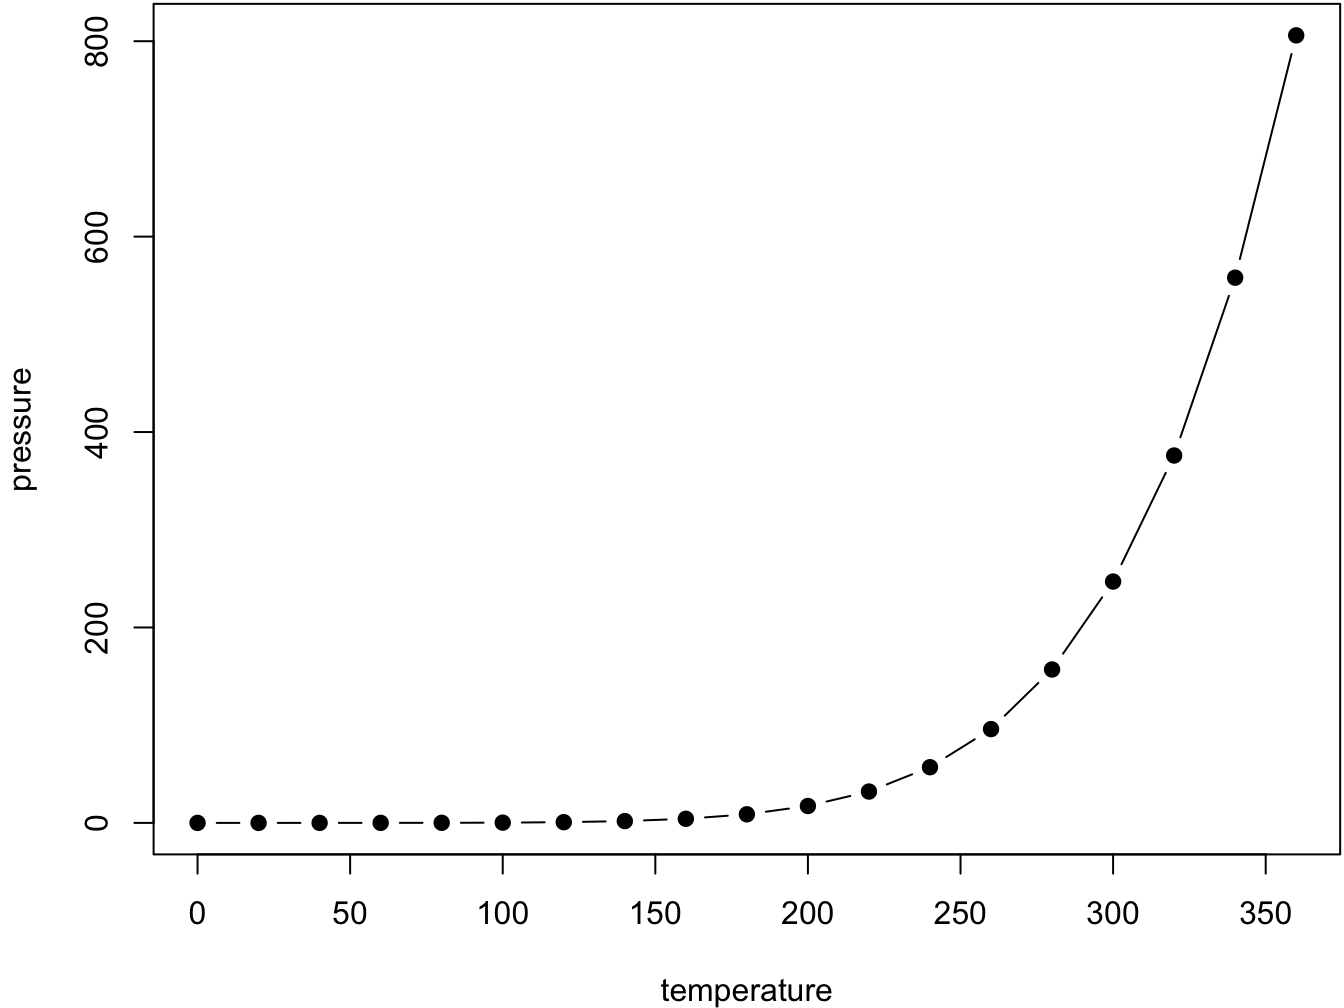
\includegraphics[width=0.8\linewidth]{ismay_kim_files/figure-latex/nice-fig-1} 

}

\caption[Here is a nice figure!]{Here is a nice figure!}\label{fig:nice-fig}
\end{figure}

Reference a figure by its code chunk label with the \texttt{fig:}
prefix, e.g., see Figure \ref{fig:nice-fig}. Similarly, you can
reference tables generated from \texttt{knitr::kable()}, e.g., see Table
\ref{tab:nice-tab}.

\begin{Shaded}
\begin{Highlighting}[]
\NormalTok{knitr::}\KeywordTok{kable}\NormalTok{(}
  \KeywordTok{head}\NormalTok{(iris, }\DecValTok{20}\NormalTok{), }\DataTypeTok{caption =} \StringTok{'Here is a nice table!'}\NormalTok{,}
  \DataTypeTok{booktabs =} \OtherTok{TRUE}
\NormalTok{)}
\end{Highlighting}
\end{Shaded}

\begin{table}

\caption{\label{tab:nice-tab}Here is a nice table!}
\centering
\begin{tabular}[t]{rrrrl}
\toprule
Sepal.Length & Sepal.Width & Petal.Length & Petal.Width & Species\\
\midrule
5.1 & 3.5 & 1.4 & 0.2 & setosa\\
4.9 & 3.0 & 1.4 & 0.2 & setosa\\
4.7 & 3.2 & 1.3 & 0.2 & setosa\\
4.6 & 3.1 & 1.5 & 0.2 & setosa\\
5.0 & 3.6 & 1.4 & 0.2 & setosa\\
\addlinespace
5.4 & 3.9 & 1.7 & 0.4 & setosa\\
4.6 & 3.4 & 1.4 & 0.3 & setosa\\
5.0 & 3.4 & 1.5 & 0.2 & setosa\\
4.4 & 2.9 & 1.4 & 0.2 & setosa\\
4.9 & 3.1 & 1.5 & 0.1 & setosa\\
\addlinespace
5.4 & 3.7 & 1.5 & 0.2 & setosa\\
4.8 & 3.4 & 1.6 & 0.2 & setosa\\
4.8 & 3.0 & 1.4 & 0.1 & setosa\\
4.3 & 3.0 & 1.1 & 0.1 & setosa\\
5.8 & 4.0 & 1.2 & 0.2 & setosa\\
\addlinespace
5.7 & 4.4 & 1.5 & 0.4 & setosa\\
5.4 & 3.9 & 1.3 & 0.4 & setosa\\
5.1 & 3.5 & 1.4 & 0.3 & setosa\\
5.7 & 3.8 & 1.7 & 0.3 & setosa\\
5.1 & 3.8 & 1.5 & 0.3 & setosa\\
\bottomrule
\end{tabular}
\end{table}

\chapter{Tidy data}\label{tidy}

\textbf{Need to give big picture question here and set up how this
chapter ties in to chapters to come}.

\textbf{Force dataframes into tibbles using \texttt{as\_tibble}? That
way \texttt{head} isn't needed since printing will be nice by default.
\url{http://r4ds.had.co.nz/tibbles.html}}

\textbf{Add RStudio graphics}

You have surely heard the word ``tidy'' in your life:

\begin{itemize}
\tightlist
\item
  ``Tidy up your room!''
\item
  ``Please write your homework in a tidy way so that it is easier to
  grade and to provide feedback.''
\item
  Marie Kondo's best-selling book
  \href{https://www.amazon.com/Life-Changing-Magic-Tidying-Decluttering-Organizing/dp/1607747308/ref=sr_1_1?ie=UTF8\&qid=1469400636\&sr=8-1\&keywords=tidying+up}{\emph{The
  Life-Changing Magic of Tidying Up: The Japanese Art of Decluttering
  and Organizing}}
\item
  ``I am not by any stretch of the imagination a tidy person, and the
  piles of unread books on the coffee table and by my bed have a
  plaintive, pleading quality to me - `Read me, please!'\,'' - Linda
  Grant
\end{itemize}

So what does it mean for your data to be \textbf{tidy}? Put simply: it
means that your data is organized. But it's more than just that. It
means that your data follows the same standard format making it easy for
others to find elements of your data, to manipulate and transform your
data, and for our purposes continuing with the common theme: it makes it
easier to visualize your data and the relationships between different
variables in your data.

\section{What is tidy data?}\label{what-is-tidy-data}

We will follow Hadley Wickham's definition of \textbf{tidy data} here
\citep{tidy}:

\begin{quote}
A dataset is a collection of values, usually either numbers (if
quantitative) or strings (if qualitative). Values are organised in two
ways. Every value belongs to a variable and an observation. A variable
contains all values that measure the same underlying attribute (like
height, temperature, duration) across units. An observation contains all
values measured on the same unit (like a person, or a day, or a race)
across attributes.
\end{quote}

\begin{quote}
Tidy data is a standard way of mapping the meaning of a dataset to its
structure. A dataset is messy or tidy depending on how rows, columns and
tables are matched up with observations, variables and types. In
\textbf{tidy data}:
\end{quote}

\begin{quote}
\begin{enumerate}
\def\labelenumi{\arabic{enumi}.}
\tightlist
\item
  Each variable forms a column.
\item
  Each observation forms a row.
\item
  Each type of observational unit forms a table.
\end{enumerate}
\end{quote}

Reading over this definition, you can begin to think about datasets that
won't follow this nice format.

\begin{center}\rule{0.5\linewidth}{\linethickness}\end{center}

\begin{learncheck}
\textbf{\emph{Learning check}}
\end{learncheck}

\textbf{(LC3.1)} Give an example dataset that doesn't follow this
format.

\begin{itemize}
\tightlist
\item
  What features of this dataset might make it difficult to visualize?\\
\item
  How could the dataset be tweaked to make it \textbf{tidy}?
\end{itemize}

\begin{center}\rule{0.5\linewidth}{\linethickness}\end{center}

\section{\texorpdfstring{The \texttt{nycflights13}
datasets}{The nycflights13 datasets}}\label{the-nycflights13-datasets}

We likely have all flown on airplanes or know someone that has. Air
travel has become an ever-present aspect of our daily lives. If you live
in or are visiting a relatively large city and you walk around that
city's airport, you see gates showing flight information from many
different airlines. And you will frequently see that some flights are
delayed because of a variety of conditions. Are there ways that we can
avoid having to deal with these flight delays?

We'd all like to arrive at our destinations on time whenever possible.
(Unless you secretly love hanging out at airports. If you are one of
these people, pretend for the moment that you are very much anticipating
being at your final destination.) Hadley Wickham (herein just referred
to as ``Hadley'') created multiple datasets containing information about
departing flights from the New York City area in 2013
\citep{R-nycflights13}. We will begin by loading in one of these
datasets, the \texttt{flights} dataset, and getting an idea of its
structure:

\begin{Shaded}
\begin{Highlighting}[]
\KeywordTok{library}\NormalTok{(nycflights13)}
\KeywordTok{data}\NormalTok{(flights)}
\end{Highlighting}
\end{Shaded}

The \texttt{library} function here loads the R package
\texttt{nycflights13} into the current R environment in which you are
working. (Note that you'll get an error if you try to load this package
in and it hasn't been installed. Check Chapter \ref{intro} to make sure
the package has been downloaded to your computer.) The next line of code
\texttt{data(flights)} loads in the \texttt{flights} dataset that is
stored in the \texttt{nycflights13} package.

This dataset and most others presented in this book will be in the
\texttt{data.frame} format in R. dataframes are ways to look at
collections of variables that are tightly coupled together. We next
begin with a couple useful R functions to get a sense for what the
\texttt{flights} dataset looks like:

\begin{Shaded}
\begin{Highlighting}[]
\KeywordTok{head}\NormalTok{(flights)}
\end{Highlighting}
\end{Shaded}

\begin{verbatim}
## # A tibble: 6 x 19
##    year month   day dep_time sched_dep_time dep_delay arr_time
##   <int> <int> <int>    <int>          <int>     <dbl>    <int>
## 1  2013     1     1      517            515         2      830
## 2  2013     1     1      533            529         4      850
## 3  2013     1     1      542            540         2      923
## 4  2013     1     1      544            545        -1     1004
## 5  2013     1     1      554            600        -6      812
## 6  2013     1     1      554            558        -4      740
## # ... with 12 more variables: sched_arr_time <int>, arr_delay <dbl>,
## #   carrier <chr>, flight <int>, tailnum <chr>, origin <chr>,
## #   dest <chr>, air_time <dbl>, distance <dbl>, hour <dbl>,
## #   minute <dbl>, time_hour <time>
\end{verbatim}

\begin{center}\rule{0.5\linewidth}{\linethickness}\end{center}

\begin{learncheck}
\textbf{\emph{Learning check}}
\end{learncheck}

\textbf{(LC3.2)} What does the \texttt{head} function give us? Why might
it be a useful function to run on a dataset you have been presented
with?

\textbf{(LC3.3)} What do you think the \texttt{tail} function would give
us for the \texttt{flights} dataset?

\textbf{(LC3.4)} What does any \emph{ONE} row in this dataset refer to?

\begin{itemize}
\tightlist
\item
  A. Data on an airline
\item
  B. Data on a flight
\item
  C. Data on an airport
\item
  D. Data on multiple flights
\end{itemize}

\begin{center}\rule{0.5\linewidth}{\linethickness}\end{center}

We see that the \texttt{head} function gives us the first six rows (by
default) for this dataset. This can give us an idea of what to expect
our dataset to look like. For example, we see the different
\textbf{variables} listed in the columns and we see that there are
different types of variables. Some of the variables like
\texttt{distance}, \texttt{day}, and \texttt{arr\_delay} are what we
will call \textbf{quantitative} variables. These variables vary in a
numerical way. Other variables here are \textbf{categorical}.

Note that if you look in the leftmost portion near the \texttt{\#\#} of
the R output, you will see a column of numbers. These are the row
numbers of the dataset. If you glance across a row with the same number,
say row 5, you can get an idea of what each row correspond to. In other
words, this will allow you to identify what object is being referred to
in a given row. This is often called the \textbf{observational unit}.
The \textbf{observational unit} in this example is an individual flight
departing New York City in 2013.

\textbf{Note}: Frequently the first thing you should do when given a
dataset is to

\begin{itemize}
\tightlist
\item
  identify the observation unit,
\item
  specify the variables, and
\item
  give the types of variables you are presented with.
\end{itemize}

\begin{Shaded}
\begin{Highlighting}[]
\KeywordTok{str}\NormalTok{(flights)}
\end{Highlighting}
\end{Shaded}

\begin{verbatim}
## Classes 'tbl_df', 'tbl' and 'data.frame':    336776 obs. of  19 variables:
##  $ year          : int  2013 2013 2013 2013 2013 2013 2013 2013 2013 2013 ...
##  $ month         : int  1 1 1 1 1 1 1 1 1 1 ...
##  $ day           : int  1 1 1 1 1 1 1 1 1 1 ...
##  $ dep_time      : int  517 533 542 544 554 554 555 557 557 558 ...
##  $ sched_dep_time: int  515 529 540 545 600 558 600 600 600 600 ...
##  $ dep_delay     : num  2 4 2 -1 -6 -4 -5 -3 -3 -2 ...
##  $ arr_time      : int  830 850 923 1004 812 740 913 709 838 753 ...
##  $ sched_arr_time: int  819 830 850 1022 837 728 854 723 846 745 ...
##  $ arr_delay     : num  11 20 33 -18 -25 12 19 -14 -8 8 ...
##  $ carrier       : chr  "UA" "UA" "AA" "B6" ...
##  $ flight        : int  1545 1714 1141 725 461 1696 507 5708 79 301 ...
##  $ tailnum       : chr  "N14228" "N24211" "N619AA" "N804JB" ...
##  $ origin        : chr  "EWR" "LGA" "JFK" "JFK" ...
##  $ dest          : chr  "IAH" "IAH" "MIA" "BQN" ...
##  $ air_time      : num  227 227 160 183 116 150 158 53 140 138 ...
##  $ distance      : num  1400 1416 1089 1576 762 ...
##  $ hour          : num  5 5 5 5 6 5 6 6 6 6 ...
##  $ minute        : num  15 29 40 45 0 58 0 0 0 0 ...
##  $ time_hour     : POSIXct, format: "2013-01-01 05:00:00" ...
\end{verbatim}

\begin{center}\rule{0.5\linewidth}{\linethickness}\end{center}

\begin{learncheck}
\textbf{\emph{Learning check}}
\end{learncheck}

\textbf{(LC3.5)} What are some examples in this dataset of
\textbf{categorical} variables? What makes them different than
\textbf{quantitative} variables?

\textbf{(LC3.6)} What does \texttt{int}, \texttt{num}, and \texttt{chr}
mean in the output above?

\textbf{(LC3.7)} How many different columns are in this dataset?

\textbf{(LC3.8)} How many different rows are in this dataset?

\begin{center}\rule{0.5\linewidth}{\linethickness}\end{center}

Another way to view the properties of a dataset is to use the
\texttt{str} function (``str'' is short for ``structure''). This will
give you the first few entries of each variable in a row after the
variable. In addition, the type of the variable is given immediately
after the \texttt{:} following each variable's name. Here, \texttt{int}
and \texttt{num} refer to quantitative variables. In contrast,
\texttt{chr} refers to categorical variables. One more type of variable
is given here with the \texttt{time\_hour} variable: \textbf{POSIXct}.
As you may suspect, this variable corresponds to a specific date and
time of day.

Another nice feature of R is the help system. You can get help in R by
simply entering a question mark before the name of a function or an
object and you will be presented with a page showing the documentation.
Note that this output help file is omitted here but can be accessed
\href{https://cran.r-project.org/web/packages/nycflights13/nycflights13.pdf}{here}
on page 3 of the PDF document.

\begin{Shaded}
\begin{Highlighting}[]
\NormalTok{?flights}
\end{Highlighting}
\end{Shaded}

Another aspect of tidy data is a description of what each variable in
the dataset represents. This helps others to understand what your
variable names mean and what they correspond to. If we look at the
output of \texttt{?flights}, we can see that a description of each
variable by name is given.

An important feature to \textbf{ALWAYS} include with your data is the
appropriate units of measurement. We'll see this further when we work
with the \texttt{dep\_delay} variable in Chapter \ref{viz}. (It's in
minutes, but you'd get some really strange interpretations if you
thought it was in hours or seconds. UNITS MATTER!)

\section{\texorpdfstring{How is \texttt{flights}
tidy?}{How is flights tidy?}}\label{how-is-flights-tidy}

We see that \texttt{flights} has a rectangular shape with each row
corresponding to a different flight and each column corresponding to a
characteristic of that flight. This matches exactly with how Hadley
defined tidy data:

\begin{enumerate}
\def\labelenumi{\arabic{enumi}.}
\tightlist
\item
  Each variable forms a column.
\item
  Each observation forms a row.
\end{enumerate}

But what about the third property?

\begin{quote}
\begin{enumerate}
\def\labelenumi{\arabic{enumi}.}
\setcounter{enumi}{2}
\tightlist
\item
  Each type of observational unit forms a table.
\end{enumerate}
\end{quote}

We identified earlier that the observational unit in the
\texttt{flights} dataset is an individual flight. And we have shown that
this dataset consists of 336776 flights with 19 variables. In other
words, some rows of this dataset don't refer to a measurement on an
airline or on an airport. They specifically refer to
characteristics/measurements on a given \textbf{flight} from New York
City in 2013.

By contrast, also included in the \texttt{nycflights13} package are
datasets with different observational units \citep{R-nycflights13}:

\begin{itemize}
\tightlist
\item
  \texttt{weather}: hourly meteorological data for each airport
\item
  \texttt{planes}: construction information about each plane
\item
  \texttt{airports}: airport names and locations
\item
  \texttt{airlines}: translation between two letter carrier codes and
  names
\end{itemize}

You may have been asking yourself what \texttt{carrier} refers to in the
\texttt{str(flights)} output above. The \texttt{airlines} dataset
provides a description of this with each airline being the observational
unit:

\begin{Shaded}
\begin{Highlighting}[]
\KeywordTok{data}\NormalTok{(airlines)}
\NormalTok{airlines}
\end{Highlighting}
\end{Shaded}

\begin{verbatim}
## # A tibble: 16 x 2
##    carrier                        name
##      <chr>                       <chr>
## 1       9E           Endeavor Air Inc.
## 2       AA      American Airlines Inc.
## 3       AS        Alaska Airlines Inc.
## 4       B6             JetBlue Airways
## 5       DL        Delta Air Lines Inc.
## 6       EV    ExpressJet Airlines Inc.
## 7       F9      Frontier Airlines Inc.
## 8       FL AirTran Airways Corporation
## 9       HA      Hawaiian Airlines Inc.
## 10      MQ                   Envoy Air
## 11      OO       SkyWest Airlines Inc.
## 12      UA       United Air Lines Inc.
## 13      US             US Airways Inc.
## 14      VX              Virgin America
## 15      WN      Southwest Airlines Co.
## 16      YV          Mesa Airlines Inc.
\end{verbatim}

\begin{Shaded}
\begin{Highlighting}[]
\KeywordTok{library}\NormalTok{(knitr)}
\KeywordTok{kable}\NormalTok{(airlines)}
\end{Highlighting}
\end{Shaded}

\begin{tabular}{l|l}
\hline
carrier & name\\
\hline
9E & Endeavor Air Inc.\\
\hline
AA & American Airlines Inc.\\
\hline
AS & Alaska Airlines Inc.\\
\hline
B6 & JetBlue Airways\\
\hline
DL & Delta Air Lines Inc.\\
\hline
EV & ExpressJet Airlines Inc.\\
\hline
F9 & Frontier Airlines Inc.\\
\hline
FL & AirTran Airways Corporation\\
\hline
HA & Hawaiian Airlines Inc.\\
\hline
MQ & Envoy Air\\
\hline
OO & SkyWest Airlines Inc.\\
\hline
UA & United Air Lines Inc.\\
\hline
US & US Airways Inc.\\
\hline
VX & Virgin America\\
\hline
WN & Southwest Airlines Co.\\
\hline
YV & Mesa Airlines Inc.\\
\hline
\end{tabular}

Note that R by default will print out the object when only its name is
given as we have done here with \texttt{airlines}. If we'd prefer to
print a dataframe out in a clean format we can use the \texttt{kable}
function in the \texttt{knitr} R package.

\section{Normal forms of data}\label{normal-forms-of-data}

The datasets included in the \texttt{nycflights13} package are in a form
that minimizes redundancy of data. We will see that there are ways to
\emph{merge} (or \emph{join}) the different tables together easily. We
are capable of doing so because each of the tables have \emph{keys} in
common to relate one to another. This is an important property of
\textbf{normal forms} of data. The process of decomposing dataframes
into less redundant tables without losing information is called
\textbf{normalization}. More information is available on
\href{https://en.wikipedia.org/wiki/Database_normalization}{Wikipedia}.

We saw an example of this above with the \texttt{airlines} dataset.
While the \texttt{flights} dataframe could also include a column with
the names of the airlines instead of the carrier code, this would be
repetitive since there is a unique mapping of the carrier code to the
name of the airline/carrier.

Below an example is given showing how to \textbf{join} the
\texttt{airlines} dataframe together with the \texttt{flights} dataframe
by linking together the two datasets via a common \textbf{key} of
\texttt{"carrier"}. Note that this ``joined'' dataframe is assigned to a
new dataframe called \texttt{joined\_flights}. The structure of
\texttt{joined\_flights} is also given so that you can see a few
elements of the new column \texttt{name} that has been added. (We will
see in Chapter \ref{manip} ways to change \texttt{name} to a more
descriptive variable name.)

\begin{Shaded}
\begin{Highlighting}[]
\KeywordTok{library}\NormalTok{(dplyr)}
\NormalTok{joined_flights <-}\StringTok{ }\KeywordTok{inner_join}\NormalTok{(}\DataTypeTok{x =} \NormalTok{flights, }\DataTypeTok{y =} \NormalTok{airlines, }\DataTypeTok{by =} \StringTok{"carrier"}\NormalTok{)}
\KeywordTok{str}\NormalTok{(joined_flights)}
\end{Highlighting}
\end{Shaded}

\begin{verbatim}
## Classes 'tbl_df', 'tbl' and 'data.frame':    336776 obs. of  20 variables:
##  $ year          : int  2013 2013 2013 2013 2013 2013 2013 2013 2013 2013 ...
##  $ month         : int  1 1 1 1 1 1 1 1 1 1 ...
##  $ day           : int  1 1 1 1 1 1 1 1 1 1 ...
##  $ dep_time      : int  517 533 542 544 554 554 555 557 557 558 ...
##  $ sched_dep_time: int  515 529 540 545 600 558 600 600 600 600 ...
##  $ dep_delay     : num  2 4 2 -1 -6 -4 -5 -3 -3 -2 ...
##  $ arr_time      : int  830 850 923 1004 812 740 913 709 838 753 ...
##  $ sched_arr_time: int  819 830 850 1022 837 728 854 723 846 745 ...
##  $ arr_delay     : num  11 20 33 -18 -25 12 19 -14 -8 8 ...
##  $ carrier       : chr  "UA" "UA" "AA" "B6" ...
##  $ flight        : int  1545 1714 1141 725 461 1696 507 5708 79 301 ...
##  $ tailnum       : chr  "N14228" "N24211" "N619AA" "N804JB" ...
##  $ origin        : chr  "EWR" "LGA" "JFK" "JFK" ...
##  $ dest          : chr  "IAH" "IAH" "MIA" "BQN" ...
##  $ air_time      : num  227 227 160 183 116 150 158 53 140 138 ...
##  $ distance      : num  1400 1416 1089 1576 762 ...
##  $ hour          : num  5 5 5 5 6 5 6 6 6 6 ...
##  $ minute        : num  15 29 40 45 0 58 0 0 0 0 ...
##  $ time_hour     : POSIXct, format: "2013-01-01 05:00:00" ...
##  $ name          : chr  "United Air Lines Inc." "United Air Lines Inc." "American Airlines Inc." "JetBlue Airways" ...
\end{verbatim}

More discussion about joining dataframes together will be given in
Chapter \ref{manip}. We will see there that the names of the columns to
be linked need not match as they did here with \texttt{"carrier"}.

\begin{center}\rule{0.5\linewidth}{\linethickness}\end{center}

\begin{center}\rule{0.5\linewidth}{\linethickness}\end{center}

\begin{review}
\textbf{\emph{Review questions}}
\end{review}

\textbf{(RQ3.1)} What are common characteristics of ``tidy'' datasets?

\textbf{(RQ3.2)} What makes ``tidy'' datasets useful for organizing
data?

\textbf{(RQ3.3)} What would the code \texttt{kable(head(flights))}
produce?

\textbf{(RQ3.4)} How many variables are presented in the table below?
What does each row correspond to? (\textbf{Hint:} You may not be able to
answer both of these questions immediately but take your best guess.)

\begin{tabular}{r|r}
\hline
students & faculty\\
\hline
4 & 2\\
\hline
6 & 3\\
\hline
\end{tabular}

\textbf{(RQ3.5)} The confusion you may have encountered in Question 4 is
a common one those that work with data are commonly presented with. This
dataset is not tidy. Actually, the dataset in Question 4 has three
variables not the two that were presented. Make a guess as to what these
variables are and present a tidy dataset instead of this untidy one
given in Question 4.

\textbf{(RQ3.6)} The actual data presented in Question 4 is given below
in tidy data format:

\begin{tabular}{l|l|l}
\hline
role & Sociology? & Type of School\\
\hline
student & TRUE & Public\\
\hline
student & TRUE & Public\\
\hline
student & TRUE & Public\\
\hline
student & TRUE & Public\\
\hline
student & FALSE & Public\\
\hline
student & FALSE & Public\\
\hline
student & FALSE & Private\\
\hline
student & FALSE & Private\\
\hline
student & FALSE & Private\\
\hline
student & FALSE & Private\\
\hline
faculty & TRUE & Public\\
\hline
faculty & TRUE & Public\\
\hline
faculty & FALSE & Public\\
\hline
faculty & FALSE & Private\\
\hline
faculty & FALSE & Private\\
\hline
\end{tabular}

\begin{itemize}
\tightlist
\item
  What does each row correspond to?\\
\item
  What are the different variables in this dataframe?\\
\item
  The \texttt{Sociology?} variable is known as a logical variable. What
  types of values does a logical variable take on?
\end{itemize}

\textbf{(RQ3.7)} What are some advantages of data in normal forms? What
are some disadvantages?

\begin{center}\rule{0.5\linewidth}{\linethickness}\end{center}

\begin{center}\rule{0.5\linewidth}{\linethickness}\end{center}

\section{What's to come?}\label{whats-to-come}

In Chapter \ref{viz}, we will further explore the distribution of a
variable in a related dataset to \texttt{flights}: the \texttt{temp}
variable in the \texttt{weather} dataset. We'll be interested in
understanding how this variable varies in relation to the values of
other variables in the dataset. We will see that visualization is often
a powerful tool in helping us see what is going on in a dataset. It will
be a useful way to expand on the \texttt{str} function we have seen here
for tidy data.

\textbf{Last updated:}

\begin{verbatim}
## [1] "Tuesday, August 02, 2016 13:47:19 CDT"
\end{verbatim}

\chapter{Visualizing Data}\label{viz}

\textbf{Compare shapes of plots instead of summary statistics?
(Berkeley)}

In Chapter \ref{tidy}, we discussed the importance of datasets being
\textbf{tidy}. You will see in examples here why having a tidy dataset
helps us immensely with plotting our data. We will focus on using
Hadley's \texttt{ggplot2} package in doing so, which was developed to
work specifically on datasets that are \textbf{tidy}. It provides an
easy way to customize your plots and is based on data visualization
theory given in \emph{The Grammar of Graphics} \citep{wilkinson2005}.

Graphics provide a nice way for us to get a sense for how quantitative
variables compare in terms of their center and their spread. It also
helps us to identify patterns and outliers in our data. We will see that
a common extension of these ideas is to compare the distribution (i.e.,
what the spread of a variable looks like) as we go across the levels of
a different categorical variable.

\section{Five Named Graphs - The FNG}\label{five-named-graphs---the-fng}

For our purposes here, we will be working with five different types of
graphs. (Note that we will use a lot of different words here in regards
to plotting - ``graphs'', ``plots'', and ``charts'' are all ways to
discuss a resulting graphic. You can think of them as all being
synonyms.) These five plots are:

\begin{itemize}
\tightlist
\item
  histograms
\item
  boxplots
\item
  barplots
\item
  scatter-plots
\item
  line-graphs
\end{itemize}

With this toolbox of plots, you can visualize just about any type of
variable thrown at you. We will discuss some other variations of these
but with the FNG in your repertoire you can do big things! Something we
will also stress here is that certain plots only work for
categorical/logical variables and others only for quantitative
variables. You'll want to quiz yourself often on which plot makes sense
with a given problem set-up.

We now introduce another dataframe in the \texttt{nycflights13} package
introduced in Chapter \ref{tidy}.

\begin{Shaded}
\begin{Highlighting}[]
\KeywordTok{library}\NormalTok{(nycflights13)}
\KeywordTok{data}\NormalTok{(weather)}
\end{Highlighting}
\end{Shaded}

\section{Histograms}\label{histograms}

Our focus now turns to the \texttt{temp} variable in this
\texttt{weather} dataset. We would like to visualize what the 26130
temperatures look like. Looking over the \texttt{weather}
dataset\footnote{To view a dataset in spreadsheet format in RStudio, you
  can run the \texttt{View()} function with the dataframe as its
  argument.} and running \texttt{?weather}, we can see that the
\texttt{temp} variable corresponds to hourly temperature (in Fahrenheit)
recordings at weather stations near airports in New York City. We could
just produce points where each of the different values appears on
something similar to a number line:

\begin{figure}
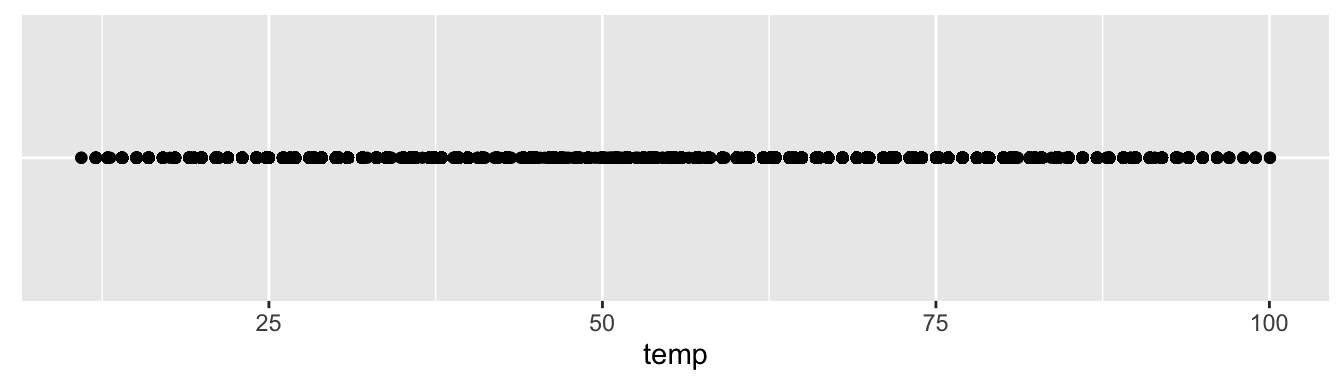
\includegraphics{ismay_kim_files/figure-latex/unnamed-chunk-12-1} \caption[Strip Plot of Hourly Temperature Recordings from NYC in 2013]{Strip Plot of Hourly Temperature Recordings from NYC in 2013}\label{fig:unnamed-chunk-12}
\end{figure}

This gives us a general idea of how the values of \texttt{temp} differ.
We see that temperatures vary from around 11 up to 100 degrees
Fahrenheit. The area between 40 and 60 degrees appears to have more
points plotted than outside that range.

What is commonly produced instead of this strip plot is a plot known as
a \textbf{histogram}. The \textbf{histogram} show how many elements of
the variable fall in specified \textbf{bins}. These \textbf{bins} may
correspond to between 0-10°F, 10-20°F, etc.

To produce a histogram, we introduce the Hadley's \texttt{ggplot2}
package \citep{R-ggplot2}. We will use the \texttt{ggplot} function
which expects at a bare minimal as arguments

\begin{itemize}
\tightlist
\item
  the dataframe where the variables exist and
\item
  the names of the variables to be plotted.
\end{itemize}

The names of the variables will be entered into the \texttt{aes}
function as arguments where \texttt{aes} stands for ``aesthetics''.

\begin{Shaded}
\begin{Highlighting}[]
\KeywordTok{ggplot}\NormalTok{(}\DataTypeTok{data =} \NormalTok{weather, }\DataTypeTok{mapping =} \KeywordTok{aes}\NormalTok{(}\DataTypeTok{x =} \NormalTok{temp))}
\end{Highlighting}
\end{Shaded}

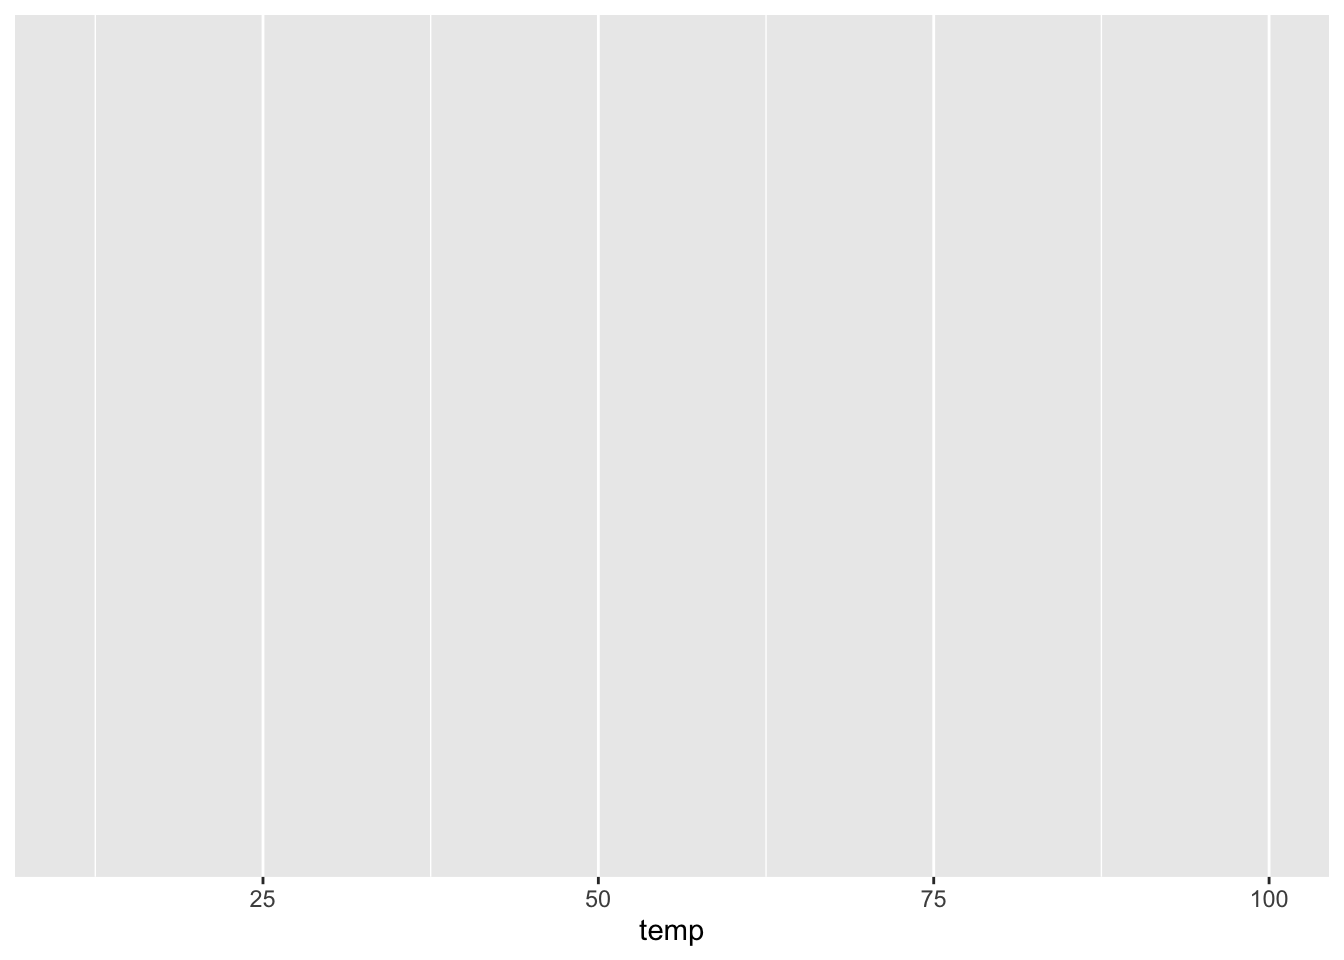
\includegraphics{ismay_kim_files/figure-latex/unnamed-chunk-13-1}

The plot given above is not a histogram, but the output does show us a
bit of what is going on with
\texttt{ggplot(data\ =\ weather,\ mapping\ =\ aes(x\ =\ temp))}. It is
producing a backdrop onto which we will ``paint'' elements.

We next proceed by adding a layer---hence, the use of the \texttt{+}
symbol---to the plot to produce a histogram. (Note also here that we
don't have to specify the \texttt{data\ =} and \texttt{mapping\ =} text
in our function calls. This is covered in more detail in Appendix A -
Chapter \ref{appendix1}.)

\begin{Shaded}
\begin{Highlighting}[]
\KeywordTok{ggplot}\NormalTok{(}\DataTypeTok{data =} \NormalTok{weather, }\DataTypeTok{mapping =} \KeywordTok{aes}\NormalTok{(}\DataTypeTok{x =} \NormalTok{temp)) +}
\StringTok{  }\KeywordTok{geom_histogram}\NormalTok{()}
\end{Highlighting}
\end{Shaded}

\begin{verbatim}
## `stat_bin()` using `bins = 30`. Pick better value with `binwidth`.
\end{verbatim}

\begin{verbatim}
## Warning: Removed 1 rows containing non-finite values (stat_bin).
\end{verbatim}

\begin{figure}
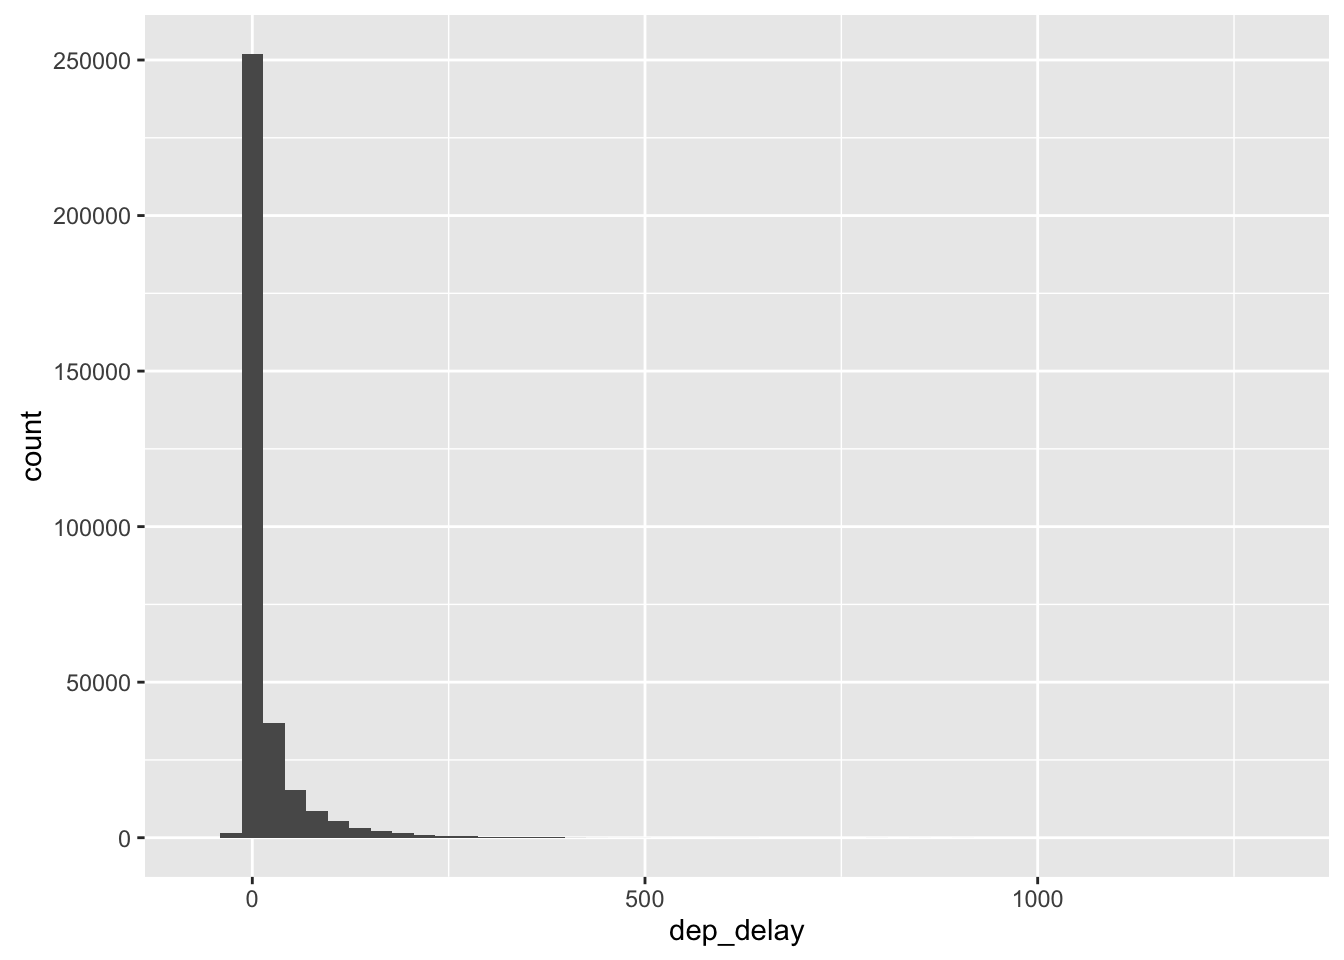
\includegraphics{ismay_kim_files/figure-latex/unnamed-chunk-14-1} \caption[Histogram of Hourly Temperature Recordings from NYC in 2013]{Histogram of Hourly Temperature Recordings from NYC in 2013}\label{fig:unnamed-chunk-14}
\end{figure}

We have the power to specify how many bins we would like to put the data
into as an argument in the \texttt{geom\_histogram} function. By
default, this is chosen to be 30 somewhat arbitrarily and we have
received a warning above our plot that this was done. We also notice
here that another warning about 1 missing value is given. This value is
omitted from the plot. This warning is ignored for future customizations
of the plot. (\textbf{Discuss missing values here?})

\begin{Shaded}
\begin{Highlighting}[]
\KeywordTok{ggplot}\NormalTok{(}\DataTypeTok{data =} \NormalTok{weather, }\DataTypeTok{mapping =} \KeywordTok{aes}\NormalTok{(}\DataTypeTok{x =} \NormalTok{temp)) +}
\StringTok{  }\KeywordTok{geom_histogram}\NormalTok{(}\DataTypeTok{bins =} \DecValTok{60}\NormalTok{)}
\end{Highlighting}
\end{Shaded}

\begin{figure}
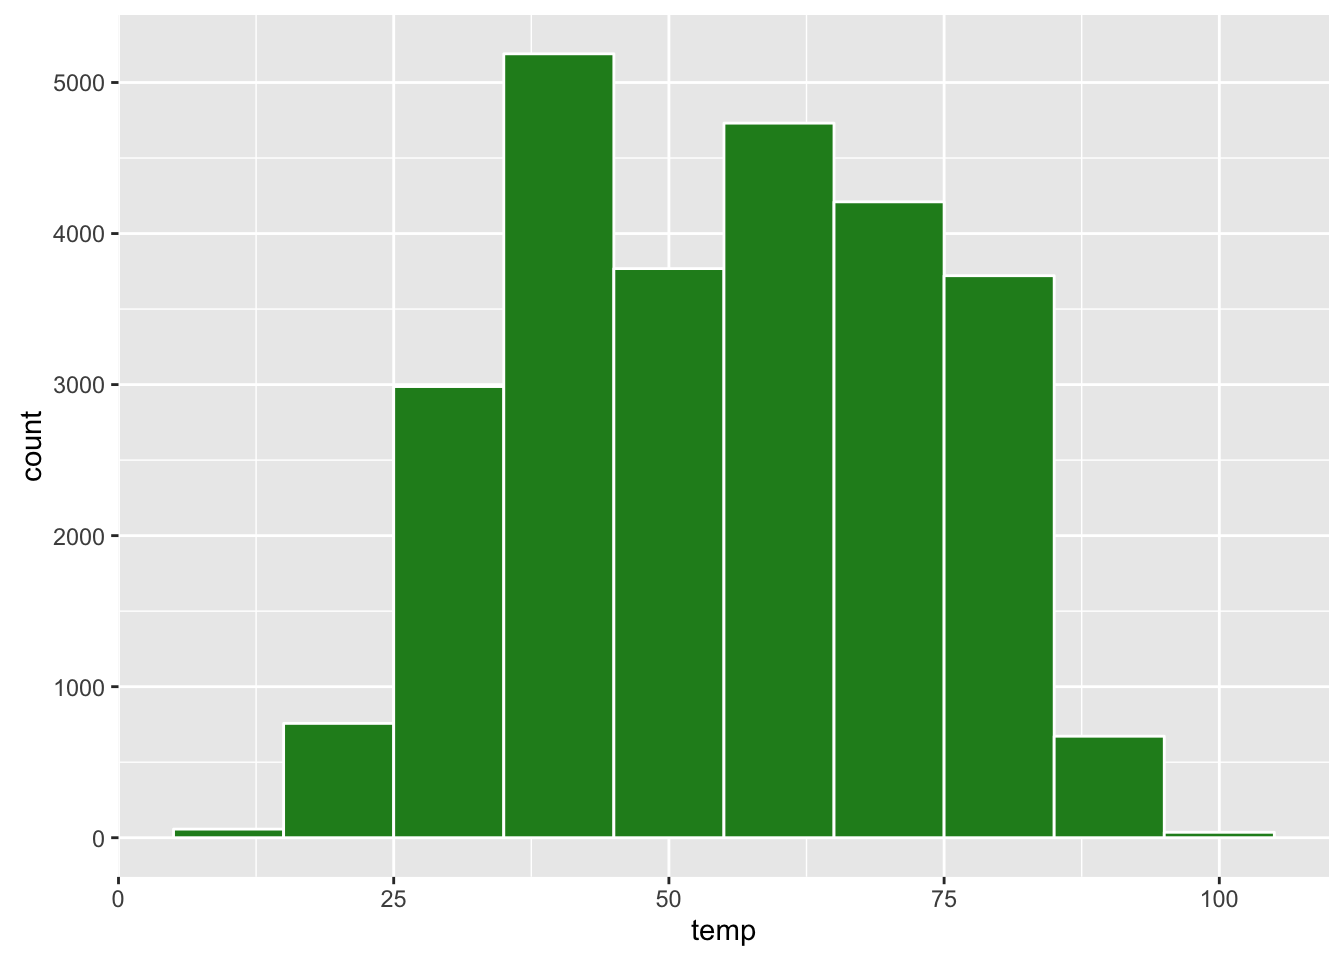
\includegraphics{ismay_kim_files/figure-latex/unnamed-chunk-15-1} \caption[Histogram of Hourly Temperature Recordings from NYC in 2013 - 60 Bins]{Histogram of Hourly Temperature Recordings from NYC in 2013 - 60 Bins}\label{fig:unnamed-chunk-15}
\end{figure}

We can tweak the plot a little more by specifying the width of the bins
(instead of how many bins to divide the variable into) by using the
\texttt{binwidth} argument in the \texttt{geom\_histogram} function. We
can also add some color to the plot by invoking the \texttt{fill} and
\texttt{color} arguments. A listing of all of the built-in colors to R
by name and color is available
\href{http://www.stat.columbia.edu/~tzheng/files/Rcolor.pdf}{here}.

\begin{Shaded}
\begin{Highlighting}[]
\KeywordTok{ggplot}\NormalTok{(}\DataTypeTok{data =} \NormalTok{weather, }\DataTypeTok{mapping =} \KeywordTok{aes}\NormalTok{(}\DataTypeTok{x =} \NormalTok{temp)) +}
\StringTok{  }\KeywordTok{geom_histogram}\NormalTok{(}\DataTypeTok{binwidth =} \DecValTok{10}\NormalTok{, }\DataTypeTok{color =} \StringTok{"white"}\NormalTok{, }\DataTypeTok{fill =} \StringTok{"forestgreen"}\NormalTok{)}
\end{Highlighting}
\end{Shaded}

\begin{figure}
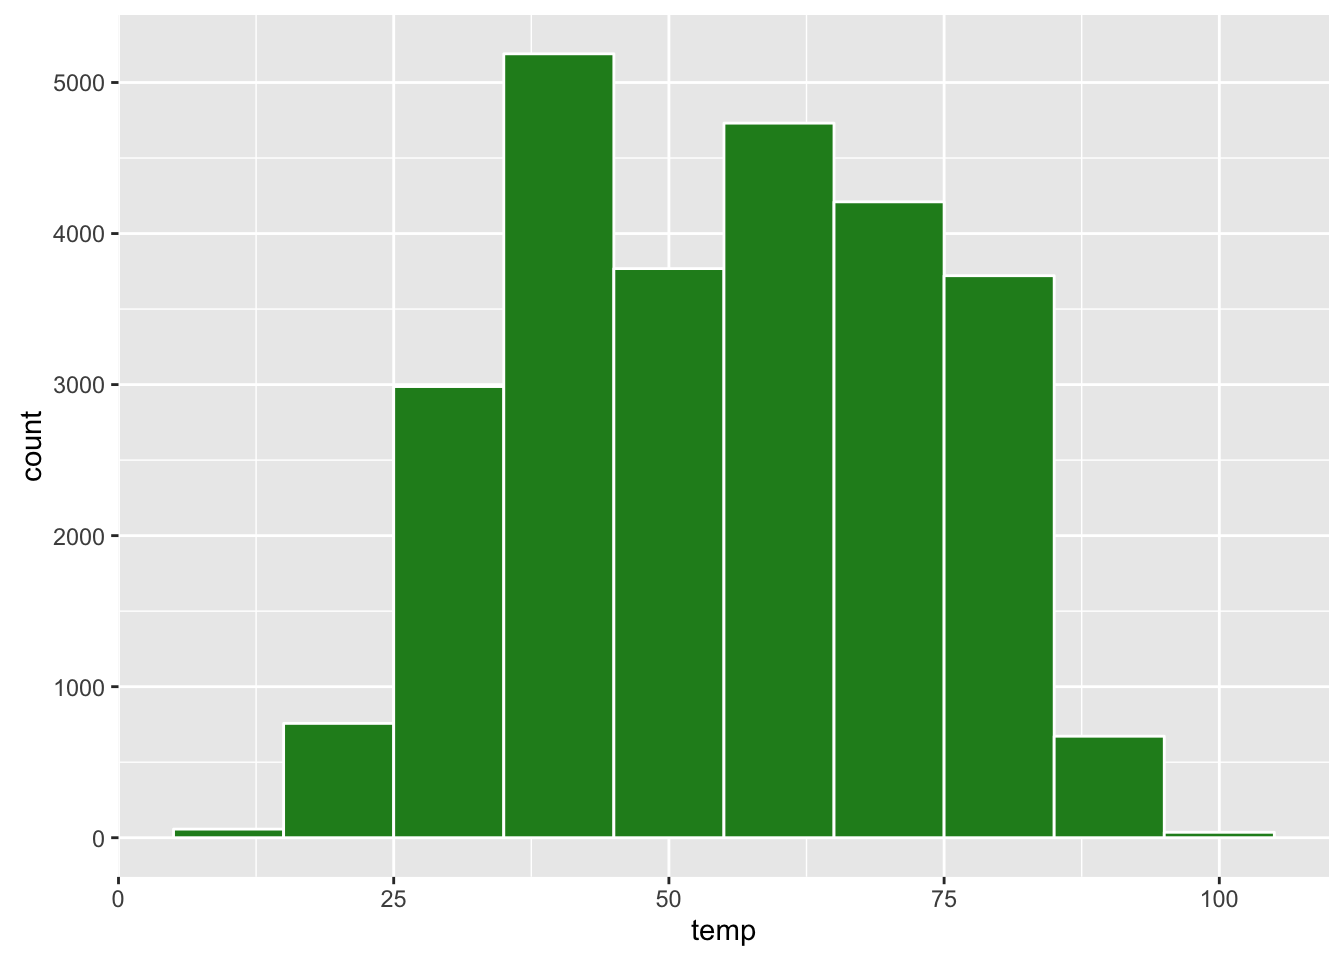
\includegraphics{ismay_kim_files/figure-latex/unnamed-chunk-16-1} \caption[Histogram of Hourly Temperature Recordings from NYC in 2013 - Binwidth = 10]{Histogram of Hourly Temperature Recordings from NYC in 2013 - Binwidth = 10}\label{fig:unnamed-chunk-16}
\end{figure}

\begin{center}\rule{0.5\linewidth}{\linethickness}\end{center}

\begin{learncheck}
\textbf{\emph{Learning check}}
\end{learncheck}

\textbf{(LC4.1)} What does changing the number of bins from 30 to 60
tell us about the distribution of temperatures?

\textbf{(LC4.2)} Would you classify the distribution of temperatures as
symmetric or skewed?

\textbf{(LC4.3)} What would you guess is the ``center'' value in this
distribution? Why did you make that choice?

\textbf{(LC4.4)} Is this data spread out greatly from the center or is
it close? Why?

\begin{center}\rule{0.5\linewidth}{\linethickness}\end{center}

\subsection{Continuous data summaries}\label{continuous-data-summaries}

The \texttt{temp} variable is a \textbf{continuous} quantitative
variable (frequently just called a \textbf{continuous variable}). ``A
variable is \textbf{continuous} if you can arrange its values in order
and an infinite number of unique values can exist between any two values
of the variable''\citep{r4ds2016}. Some common examples of continuous
variables are time and height. Between any two times there are an
infinitely many number of time units that fall between them.

It is often easier to think about quantitative variables that are not
continuous to help us better understand continuity. The best example is
counts. If we are looking to count the number of flights that depart on
a given day from New York City, this variable would not be continuous.
It falls on a \textbf{discrete} scale.

We can examine some summary information about this \texttt{temp}
variable. To do so, we introduce the \texttt{summary} function. (We will
see in Chapter \ref{manip} how to use the \texttt{summarize} function in
the \texttt{dplyr} package to produce similar results.)

The syntax here is a little different than what we have seen before. (A
further discussion about R syntax is available in Appendix A - Chapter
\ref{appendix1}). Here, \texttt{summary} is the function and it is
expecting an object to be summarized as its argument. The object here is
the \texttt{temp} variable in the \texttt{weather} dataframe. To focus
on just this one variable \texttt{temp} in \texttt{weather}, we separate
them by the dollar sign symbol \texttt{\$}. Order matters here: the
dataframe comes before the \texttt{\$} and the variable/column name
comes after.

\begin{Shaded}
\begin{Highlighting}[]
\KeywordTok{summary}\NormalTok{(weather$temp)}
\end{Highlighting}
\end{Shaded}

\begin{verbatim}
##    Min. 1st Qu.  Median    Mean 3rd Qu.    Max.    NA's 
##   10.94   39.92   55.04   55.20   69.98  100.00       1
\end{verbatim}

This tells us what is known as the \textbf{five-number summary} for our
variable as well as the \textbf{mean} value of the variable. More
information on both of these concepts is given in Appendix A - Chapter
\ref{appendix1}.

This \texttt{summary} gives us some numerical summaries of our
temperature variable. The minimum recorded temperature is 10.94 degrees
Fahrenheit and the maximum is 100.04 degrees Fahrenheit. We have one
missing value denoted as an \texttt{NA} in the observations of this
variable. The median Fahrenheit temperature of 55.04 and mean of
55.2035149 are quite close. This is a property of symmetric
distributions.

The last two entries given by \texttt{summary} correspond to the
25\textsuperscript{th} percentile and the 75\textsuperscript{th}
percentile. If we sorted all of the temperatures in increasing order, we
would see that 25\% of them would fall below 39.92 and that 75\% of them
would fall below 69.98. This implies that the middle 50\% of data values
lie between 39.92 and 69.98 degrees Fahrenheit.

\textbf{Introduce standard deviation here?}

\subsection{Summary}\label{summary}

Histograms provide a useful way of looking at how ONE continuous
variable varies. They allow us to answer questions such as

\begin{itemize}
\tightlist
\item
  Are there values far away from the center? These are commonly called
  \textbf{outliers} and can frequently be easily identified on a
  histogram.
\item
  Are most values close to the center? If so, the spread of the variable
  is small. If not, the spread is large.
\item
  How spread out are the values? One measure of this spread is
  \textbf{standard deviation} discussed above.
\end{itemize}

The histogram show how many entries fall in different groupings of this
variable. Another common property of distributions is symmetry and as we
saw it is quite easily identified by looking over the histogram produced
from the variable's values.

\section{Boxplots}\label{boxplots}

Histograms can also be produced to compare the distribution of a
variable over another variable. Suppose we were interested in looking at
how the temperature recordings we saw in the last section varied by
month. This is what is meant by ``the distribution of a variable over
another variable'': \texttt{temp} is one variable and \texttt{month} is
the other variable.

\subsection{Faceting}\label{faceting}

In order to look at histograms of \texttt{temp} for each month, we
introduce a new concept called \textbf{facetting}. Faceting is used when
we'd like to create small multiples of the same plot over a different
categorical variable. By default, all of the small multiples will have
the same vertical axis. An example will help here. We will discuss the
concept of faceting in further detail in Section \ref{barplots}.

\begin{Shaded}
\begin{Highlighting}[]
\KeywordTok{ggplot}\NormalTok{(}\DataTypeTok{data =} \NormalTok{weather, }\DataTypeTok{mapping =} \KeywordTok{aes}\NormalTok{(}\DataTypeTok{x =} \NormalTok{temp)) +}
\StringTok{  }\KeywordTok{geom_histogram}\NormalTok{(}\DataTypeTok{binwidth =} \DecValTok{5}\NormalTok{, }\DataTypeTok{color =} \StringTok{"white"}\NormalTok{, }\DataTypeTok{fill =} \StringTok{"firebrick"}\NormalTok{) +}
\StringTok{  }\KeywordTok{facet_wrap}\NormalTok{(~month)}
\end{Highlighting}
\end{Shaded}

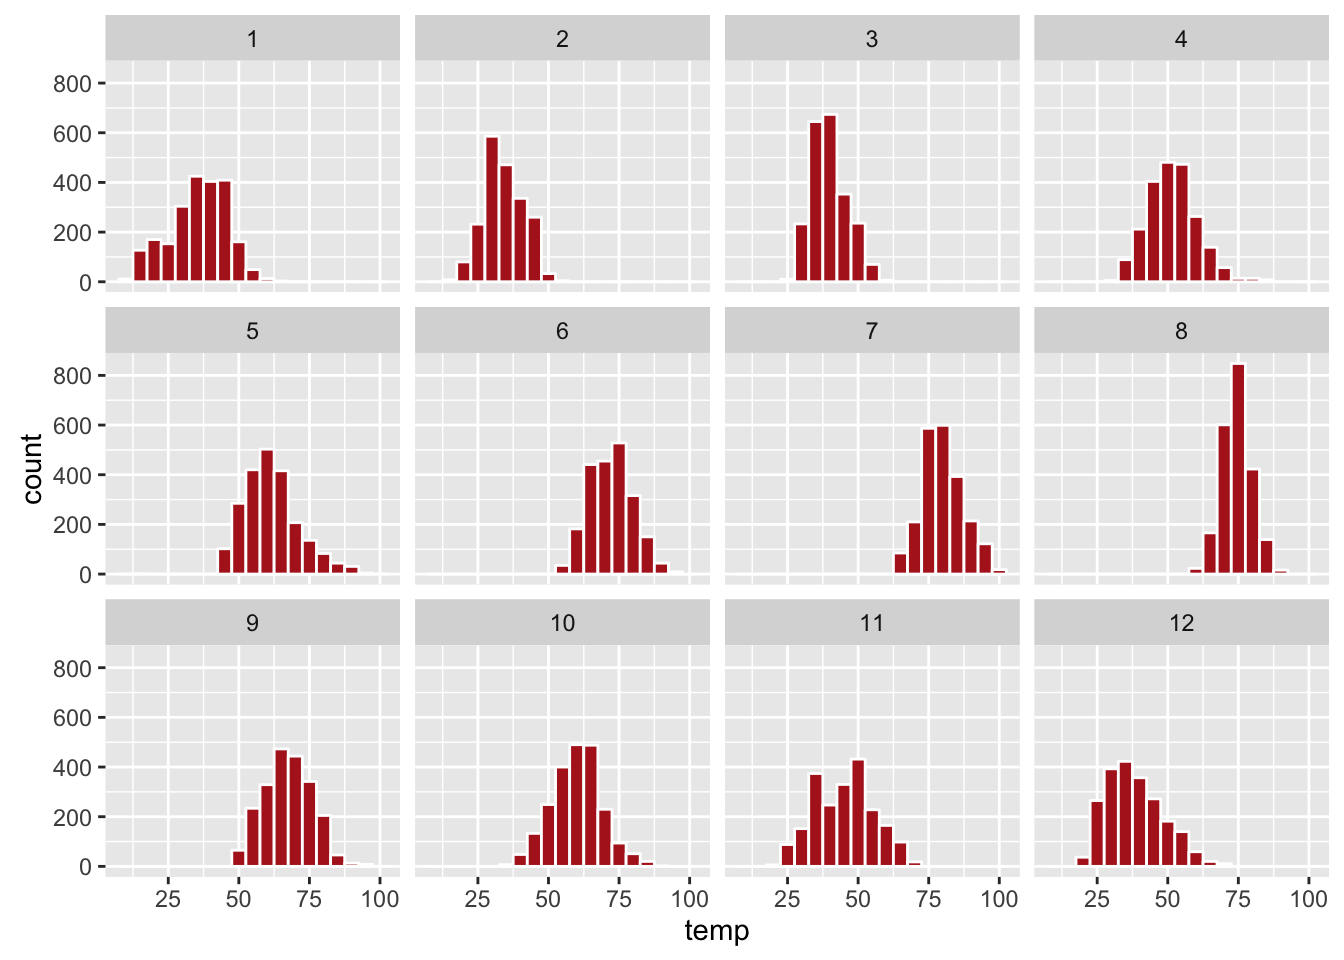
\includegraphics{ismay_kim_files/figure-latex/unnamed-chunk-18-1}

As we might expect, the temperature tends to increase as summer
approaches and then decrease as winter approaches.

\begin{center}\rule{0.5\linewidth}{\linethickness}\end{center}

\begin{learncheck}
\textbf{\emph{Learning check}}
\end{learncheck}

\textbf{(LC4.5)} What other things do you notice about the faceted plot
above? How does a faceted plot help us see how relationships between two
variables?

\textbf{(LC4.6)} What do the numbers 1-12 correspond to in the plot
above? What about 25, 50, 75, 100?

\textbf{(LC4.7)} What could be done to make the faceted plot above more
readable? (Focus on tweaking the histograms and not on making a
different type of plot here.)

\textbf{(LC4.8)} For which types of datasets would these types of
faceted plots not work well in comparing relationships between
variables? Draw or give an example.

\begin{center}\rule{0.5\linewidth}{\linethickness}\end{center}

Histograms can provide a way to compare distributions across groups as
we see above when we looked at temperature over months. Frequently, a
plot called a \textbf{boxplot} (also called a \textbf{side-by-side
boxplot}) is done instead. The \textbf{boxplot} uses the information
provided in the \textbf{five-number summary} referred to in the previous
section when we used the \texttt{summary} function. It gives a way to
compare this summary information across the different levels of a group.
Let's create a boxplot to compare the monthly temperatures as we did
above with the faceted histograms.

\begin{Shaded}
\begin{Highlighting}[]
\KeywordTok{ggplot}\NormalTok{(}\DataTypeTok{data =} \NormalTok{weather, }\DataTypeTok{mapping =} \KeywordTok{aes}\NormalTok{(}\DataTypeTok{x =} \NormalTok{month, }\DataTypeTok{y =} \NormalTok{temp)) +}
\StringTok{  }\KeywordTok{geom_boxplot}\NormalTok{()}
\end{Highlighting}
\end{Shaded}

\begin{verbatim}
## Warning: Continuous x aesthetic -- did you forget aes(group=...)?
\end{verbatim}

\begin{verbatim}
## Warning: Removed 1 rows containing non-finite values (stat_boxplot).
\end{verbatim}

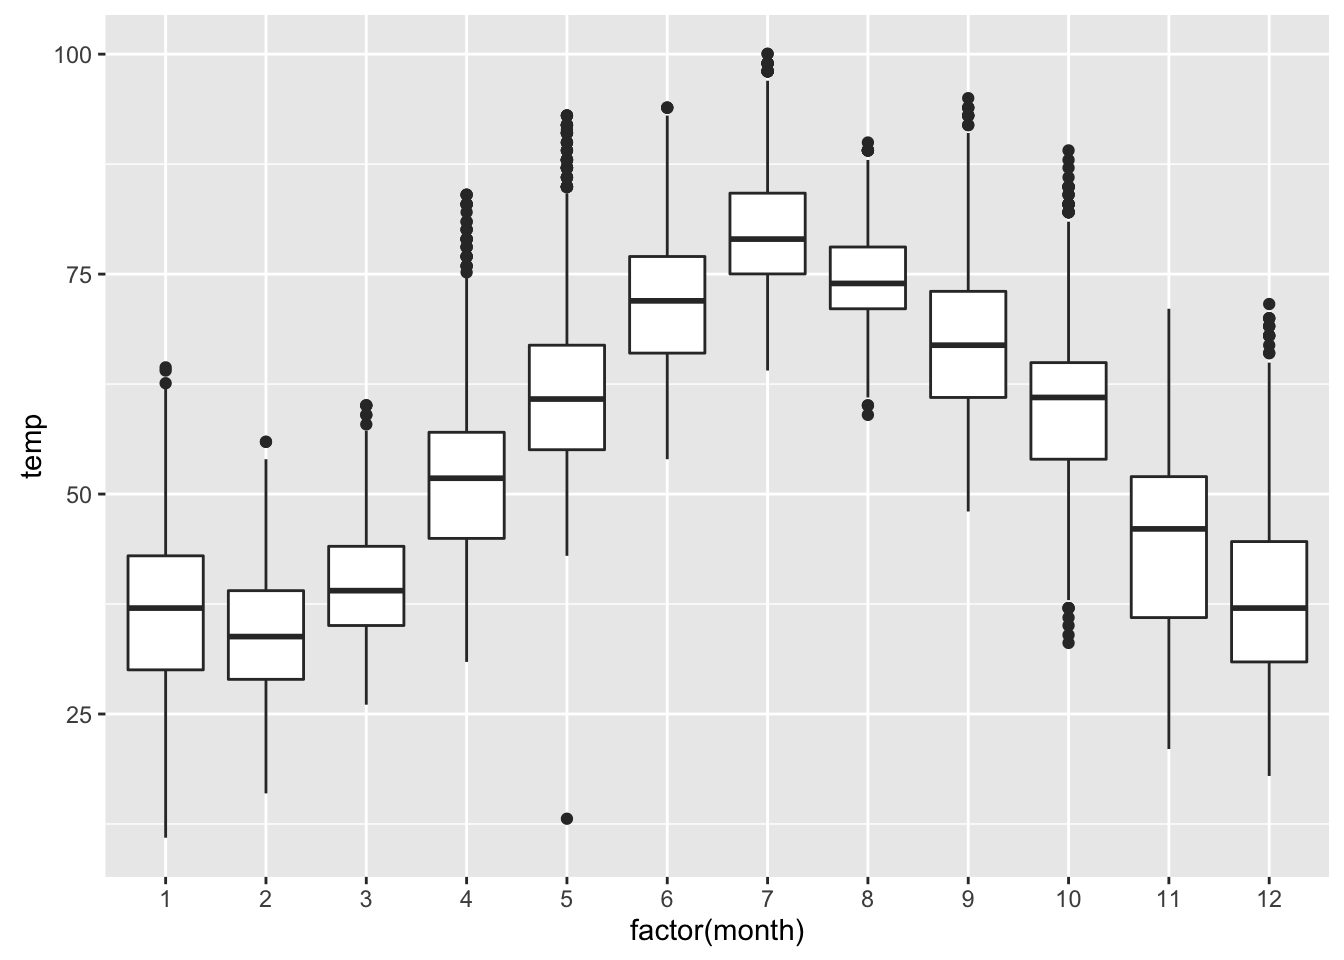
\includegraphics{ismay_kim_files/figure-latex/unnamed-chunk-19-1}

Note the first warning that is given here. (The second one corresponds
to missing values in the dataframe and it is turned off on subsequent
plots.) This plot does not look like what we were expecting. We were
expecting to see the distribution of temperatures for each month (so 12
different boxplots). This gives us the overall boxplot without any other
groupings. We can get around this by introducing a new function for our
\texttt{x} variable.

\begin{Shaded}
\begin{Highlighting}[]
\KeywordTok{ggplot}\NormalTok{(}\DataTypeTok{data =} \NormalTok{weather, }\DataTypeTok{mapping =} \KeywordTok{aes}\NormalTok{(}\DataTypeTok{x =} \KeywordTok{factor}\NormalTok{(month), }\DataTypeTok{y =} \NormalTok{temp)) +}
\StringTok{  }\KeywordTok{geom_boxplot}\NormalTok{()}
\end{Highlighting}
\end{Shaded}

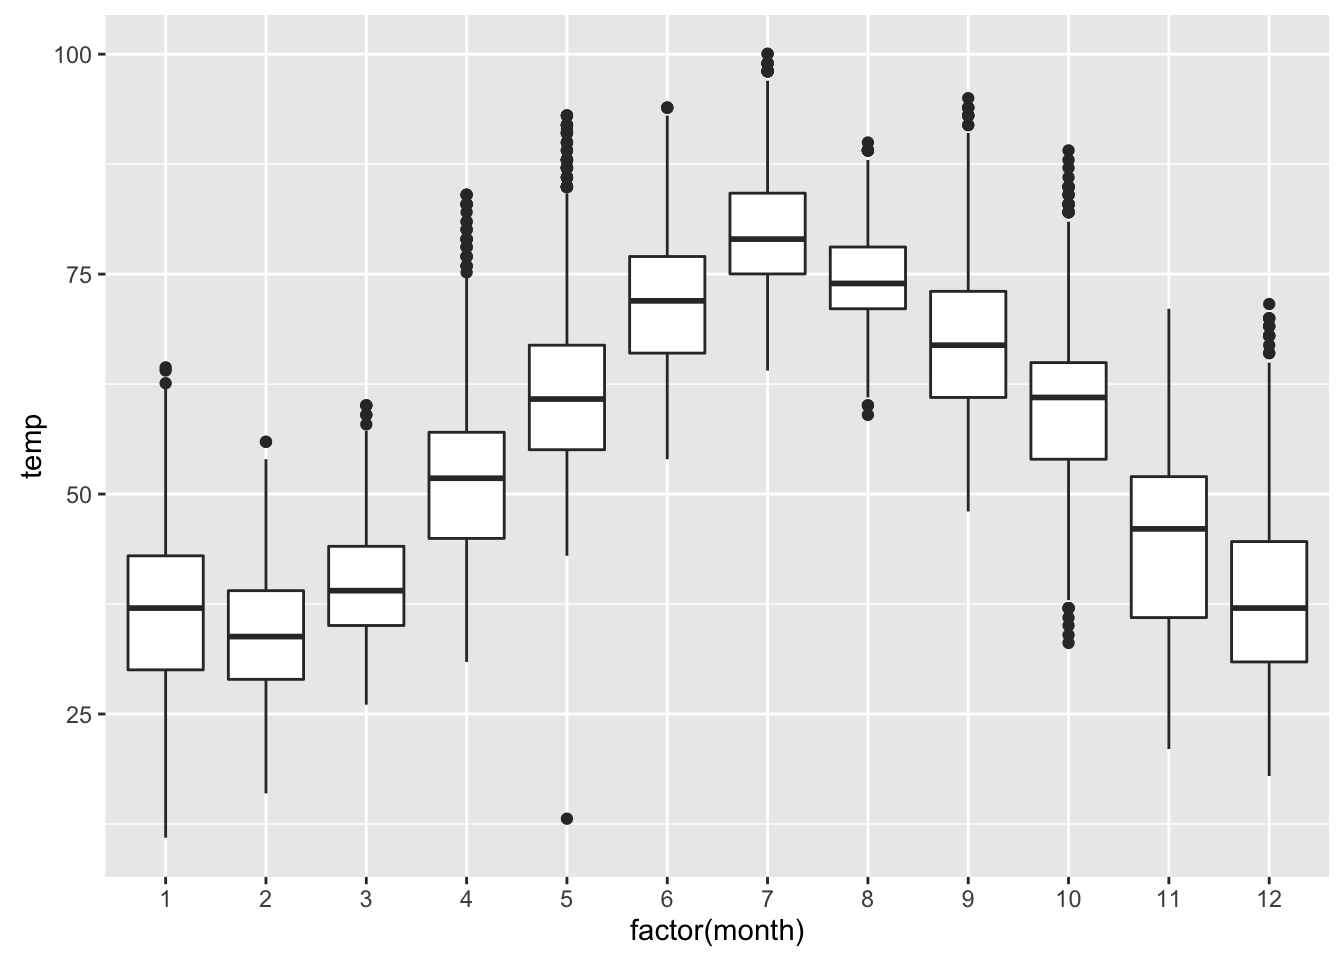
\includegraphics{ismay_kim_files/figure-latex/unnamed-chunk-20-1}

We have introduced a new function called \texttt{factor()} here. One of
the things this function does is to convert a numeric value like
\texttt{month} (1, 2, \ldots{}, 12) into a categorical variable. The
``box'' part of this plot represents the 25\textsuperscript{th}
percentile, the median (50\textsuperscript{th} percentile), and the
75\textsuperscript{th} percentile. The dots correspond to
\textbf{outliers}. (The specific formulation for these outliers is
discussed in Appendix A - Chapter \ref{appendix1}.) The lines show how
the data varies that is not in the center 50\% defined by the first and
third quantiles. Longer lines correspond to more variability and shorter
lines correspond to less variability.

\begin{center}\rule{0.5\linewidth}{\linethickness}\end{center}

\begin{learncheck}
\textbf{\emph{Learning check}}
\end{learncheck}

\textbf{(LC4.9)} What does the dot at the bottom of the plot for May
correspond to? Explain what might have occurred in May to produce this
point.

\textbf{(LC4.10)} Which months have the highest variability in
temperature? What reasons do you think this is?

\textbf{(LC4.11)} We looked at the distribution of a continuous variable
over a categorical variable here with this boxplot. Why can't we look at
the distribution of one continuous variable over the distribution of
another continuous variable? Say temperature across pressure, for
example?

\textbf{(LC4.12)} Boxplots provide a simple way to identify outliers.
Why may outliers be easier to identify when looking at a boxplot instead
of a faceted histogram?

\begin{center}\rule{0.5\linewidth}{\linethickness}\end{center}

\subsection{Summary}\label{summary-1}

Boxplots provide a way to compare and contrast the distribution of ONE
quantitative variable across multiple levels of ONE categorical
variable. One can easily look to see where the median falls across the
different groups by looking at the center line in the box. You can also
see how spread out the variable is across the different groups by
looking at the width of the box and also how far out the lines stretch
from the box. Lastly, outliers are even more easily identified when
looking at a boxplot than when looking at a histogram.

\section{Barplots}\label{barplots}

Both histograms and boxplots represent ways to visualize the variability
of continuous variables. Another common task is to present the
distribution of a categorical variable. This is a simpler task since we
will be interested in how many elements from our data fall into the
different categories of the categorical variable. We need not bin the
data or identify the different quantiles for categorical variables.

Frequently, the best way to visualize these different counts (also known
as \textbf{frequencies}) is via a barplot. Consider the distribution of
airlines that flew out of New York City in 2013. This can be plotted by
invoking the \texttt{geom\_bar} function in \texttt{ggplot2}:

\begin{Shaded}
\begin{Highlighting}[]
\KeywordTok{ggplot}\NormalTok{(}\DataTypeTok{data =} \NormalTok{flights, }\DataTypeTok{mapping =} \KeywordTok{aes}\NormalTok{(}\DataTypeTok{x =} \NormalTok{carrier)) +}
\StringTok{  }\KeywordTok{geom_bar}\NormalTok{()}
\end{Highlighting}
\end{Shaded}

\begin{figure}
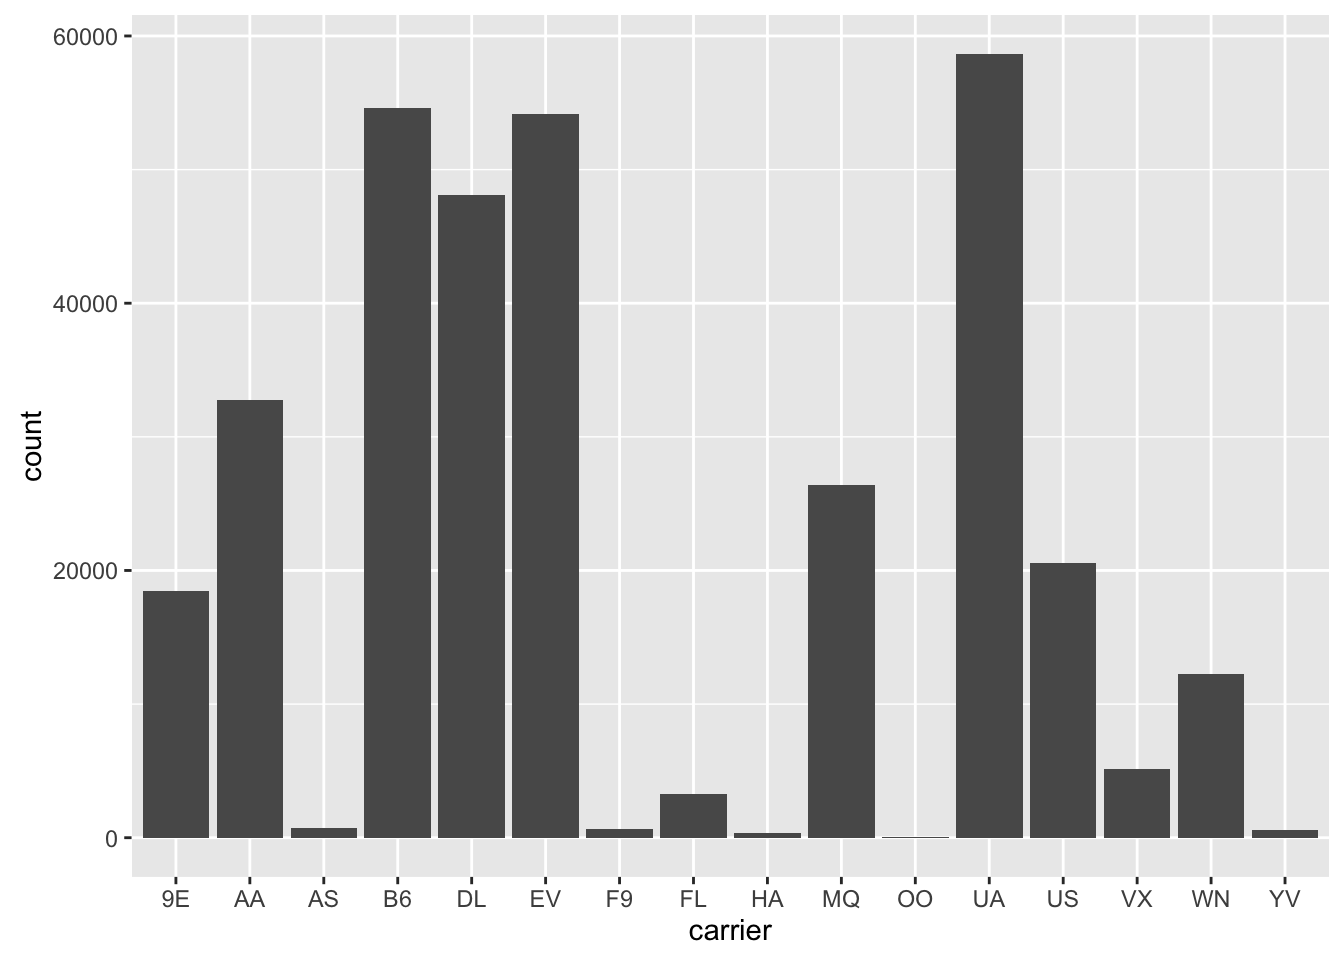
\includegraphics{ismay_kim_files/figure-latex/unnamed-chunk-21-1} \caption[Number of flights departing NYC in 2013 by airline]{Number of flights departing NYC in 2013 by airline}\label{fig:unnamed-chunk-21}
\end{figure}

Recall the \texttt{airlines} dataset discussed in Chapter \ref{tidy}.

\begin{Shaded}
\begin{Highlighting}[]
\KeywordTok{library}\NormalTok{(knitr)}
\KeywordTok{data}\NormalTok{(airlines)}
\KeywordTok{kable}\NormalTok{(airlines)}
\end{Highlighting}
\end{Shaded}

\begin{tabular}{l|l}
\hline
carrier & name\\
\hline
9E & Endeavor Air Inc.\\
\hline
AA & American Airlines Inc.\\
\hline
AS & Alaska Airlines Inc.\\
\hline
B6 & JetBlue Airways\\
\hline
DL & Delta Air Lines Inc.\\
\hline
EV & ExpressJet Airlines Inc.\\
\hline
F9 & Frontier Airlines Inc.\\
\hline
FL & AirTran Airways Corporation\\
\hline
HA & Hawaiian Airlines Inc.\\
\hline
MQ & Envoy Air\\
\hline
OO & SkyWest Airlines Inc.\\
\hline
UA & United Air Lines Inc.\\
\hline
US & US Airways Inc.\\
\hline
VX & Virgin America\\
\hline
WN & Southwest Airlines Co.\\
\hline
YV & Mesa Airlines Inc.\\
\hline
\end{tabular}

We see that United Air Lines, JetBlue Airways, and ExpressJet Airlines
had the most flights depart New York City in 2013. To get the actual
number of flights by each airline we can use the \texttt{table} function
on the \texttt{carrier} variable in \texttt{flights}:

\begin{Shaded}
\begin{Highlighting}[]
\NormalTok{flights_table <-}\StringTok{ }\KeywordTok{table}\NormalTok{(flights$carrier)}
\NormalTok{flights_table}
\end{Highlighting}
\end{Shaded}

\begin{verbatim}
## 
##    9E    AA    AS    B6    DL    EV    F9    FL    HA    MQ    OO    UA 
## 18460 32729   714 54635 48110 54173   685  3260   342 26397    32 58665 
##    US    VX    WN    YV 
## 20536  5162 12275   601
\end{verbatim}

More information on the use of this \texttt{\$} syntax is available in
Chapter \ref{tidy} and in Appendix A - Chapter \ref{appendix1}.

\begin{center}\rule{0.5\linewidth}{\linethickness}\end{center}

\begin{learncheck}
\textbf{\emph{Learning check}}
\end{learncheck}

\textbf{(LC4.13)} Why are histograms inappropriate for visualizing
categorical variables?

\textbf{(LC4.14)} What is the difference between histograms and
barplots?

\textbf{(LC4.15)} How many Envoy Air flights departed NYC in 2013?

\textbf{(LC4.16)} What was the seventh highest airline in terms of
departed flights from NYC in 2013?

\begin{center}\rule{0.5\linewidth}{\linethickness}\end{center}

\subsection{Must avoid pie charts!}\label{must-avoid-pie-charts}

Unfortunately, one of the most common plots seen today for categorical
data is the pie chart. While they may see harmless enough, they actually
present a problem in that humans are unable to judge angles well. As
Naomi Robbins describes in her book ``Creating More Effective Graphs'',
we overestimate angles greater than 90 degrees and we underestimate
angles less than 90 degrees. In other words, it is difficult for us to
determine relative size of one piece of the pie compared to another.

Let's examine our previous barplot example on the number of flights
departing NYC by airline. This time we will use a pie chart. As you
review this chart, try to identify

\begin{itemize}
\tightlist
\item
  how much larger the portion of the pie is for ExpressJet Airlines
  (\texttt{EV}) compared to US Airways (\texttt{US}),
\item
  what the third largest carrier is in terms of departing flights, and
\item
  how many carriers have fewer flights than United Airlines
  (\texttt{UA})?
\end{itemize}

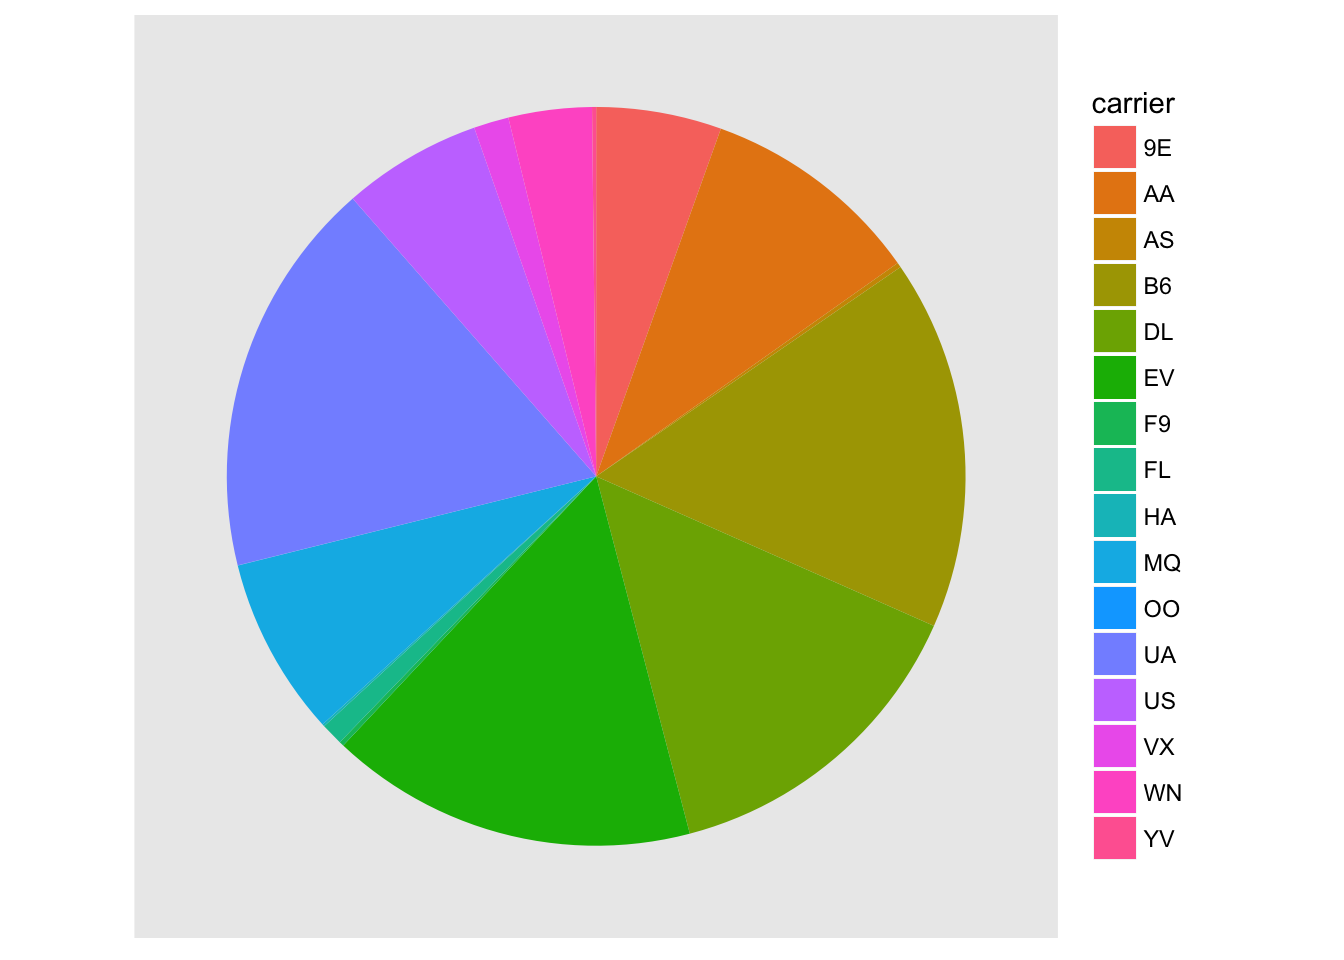
\includegraphics{ismay_kim_files/figure-latex/unnamed-chunk-24-1}

While it is quite easy to look back at the barplot to get the answer to
these questions, it's quite difficult to get the answers correct when
looking at the pie graph. Barplots can always present the information in
a way that is easier for the eye to determine relative position. There
may be one exception from Nathan Yau at
\href{https://flowingdata.com/2008/09/19/pie-i-have-eaten-and-pie-i-have-not-eaten/}{FlowingData.com}
but we will leave this for the reader to decide:

\begin{center}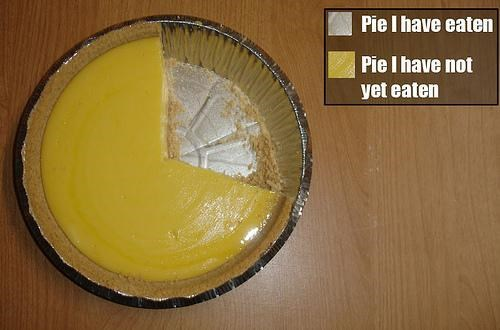
\includegraphics[width=6.94in]{images/Pie-I-have-Eaten} \end{center}

\begin{center}\rule{0.5\linewidth}{\linethickness}\end{center}

\begin{learncheck}
\textbf{\emph{Learning check}}
\end{learncheck}

\textbf{(LC4.17)} Why should pie charts be avoided and replaced by
barplots?

\textbf{(LC4.18)} What is your opinion as to why pie charts continue to
be used?

\begin{center}\rule{0.5\linewidth}{\linethickness}\end{center}

\subsection{Using barplots to compare two
variables}\label{using-barplots-to-compare-two-variables}

Barplots are the go-to way to visualize the frequency of different
categories of a categorical variable. They make it easy to order the
counts and to compare one group's frequency to another. Another use of
barplots (unfortunately, sometimes inappropriately and confusingly) is
to compare two categorical variables together. Let's examine the
distribution of outgoing flights from NYC by \texttt{carrier} and
\texttt{airport}.

We begin by getting the names of the airports in NYC that were included
in the \texttt{flights} dataset. Remember from Chapter \ref{tidy} that
this can be done by using the \texttt{inner\_join} function in the
\texttt{dplyr} package.

\begin{Shaded}
\begin{Highlighting}[]
\KeywordTok{library}\NormalTok{(dplyr)}
\NormalTok{flights_namedports <-}\StringTok{ }\KeywordTok{inner_join}\NormalTok{(flights, airports, }\DataTypeTok{by =} \KeywordTok{c}\NormalTok{(}\StringTok{"origin"} \NormalTok{=}\StringTok{ "faa"}\NormalTok{))}
\KeywordTok{str}\NormalTok{(flights_namedports)}
\end{Highlighting}
\end{Shaded}

\begin{verbatim}
## Classes 'tbl_df', 'tbl' and 'data.frame':    336776 obs. of  25 variables:
##  $ year          : int  2013 2013 2013 2013 2013 2013 2013 2013 2013 2013 ...
##  $ month         : int  1 1 1 1 1 1 1 1 1 1 ...
##  $ day           : int  1 1 1 1 1 1 1 1 1 1 ...
##  $ dep_time      : int  517 533 542 544 554 554 555 557 557 558 ...
##  $ sched_dep_time: int  515 529 540 545 600 558 600 600 600 600 ...
##  $ dep_delay     : num  2 4 2 -1 -6 -4 -5 -3 -3 -2 ...
##  $ arr_time      : int  830 850 923 1004 812 740 913 709 838 753 ...
##  $ sched_arr_time: int  819 830 850 1022 837 728 854 723 846 745 ...
##  $ arr_delay     : num  11 20 33 -18 -25 12 19 -14 -8 8 ...
##  $ carrier       : chr  "UA" "UA" "AA" "B6" ...
##  $ flight        : int  1545 1714 1141 725 461 1696 507 5708 79 301 ...
##  $ tailnum       : chr  "N14228" "N24211" "N619AA" "N804JB" ...
##  $ origin        : chr  "EWR" "LGA" "JFK" "JFK" ...
##  $ dest          : chr  "IAH" "IAH" "MIA" "BQN" ...
##  $ air_time      : num  227 227 160 183 116 150 158 53 140 138 ...
##  $ distance      : num  1400 1416 1089 1576 762 ...
##  $ hour          : num  5 5 5 5 6 5 6 6 6 6 ...
##  $ minute        : num  15 29 40 45 0 58 0 0 0 0 ...
##  $ time_hour     : POSIXct, format: "2013-01-01 05:00:00" ...
##  $ name          : chr  "Newark Liberty Intl" "La Guardia" "John F Kennedy Intl" "John F Kennedy Intl" ...
##  $ lat           : num  40.7 40.8 40.6 40.6 40.8 ...
##  $ lon           : num  -74.2 -73.9 -73.8 -73.8 -73.9 ...
##  $ alt           : int  18 22 13 13 22 18 18 22 13 22 ...
##  $ tz            : num  -5 -5 -5 -5 -5 -5 -5 -5 -5 -5 ...
##  $ dst           : chr  "A" "A" "A" "A" ...
\end{verbatim}

We see that \texttt{name} now corresponds to the name of the airport as
referenced by the \texttt{origin} variable. We will now plot
\texttt{carrier} as the horizontal variable. When we specify
\texttt{geom\_bar}, it will specify \texttt{count} as being the vertical
variable. A new addition here is \texttt{fill\ =\ name}. Look over what
was produced from the plot to get an idea of what this argument gives.

\begin{Shaded}
\begin{Highlighting}[]
\KeywordTok{ggplot}\NormalTok{(}\DataTypeTok{data =} \NormalTok{flights_namedports, }\DataTypeTok{mapping =} \KeywordTok{aes}\NormalTok{(}\DataTypeTok{x =} \NormalTok{carrier, }\DataTypeTok{fill =} \NormalTok{name)) +}
\StringTok{  }\KeywordTok{geom_bar}\NormalTok{()}
\end{Highlighting}
\end{Shaded}

\begin{figure}
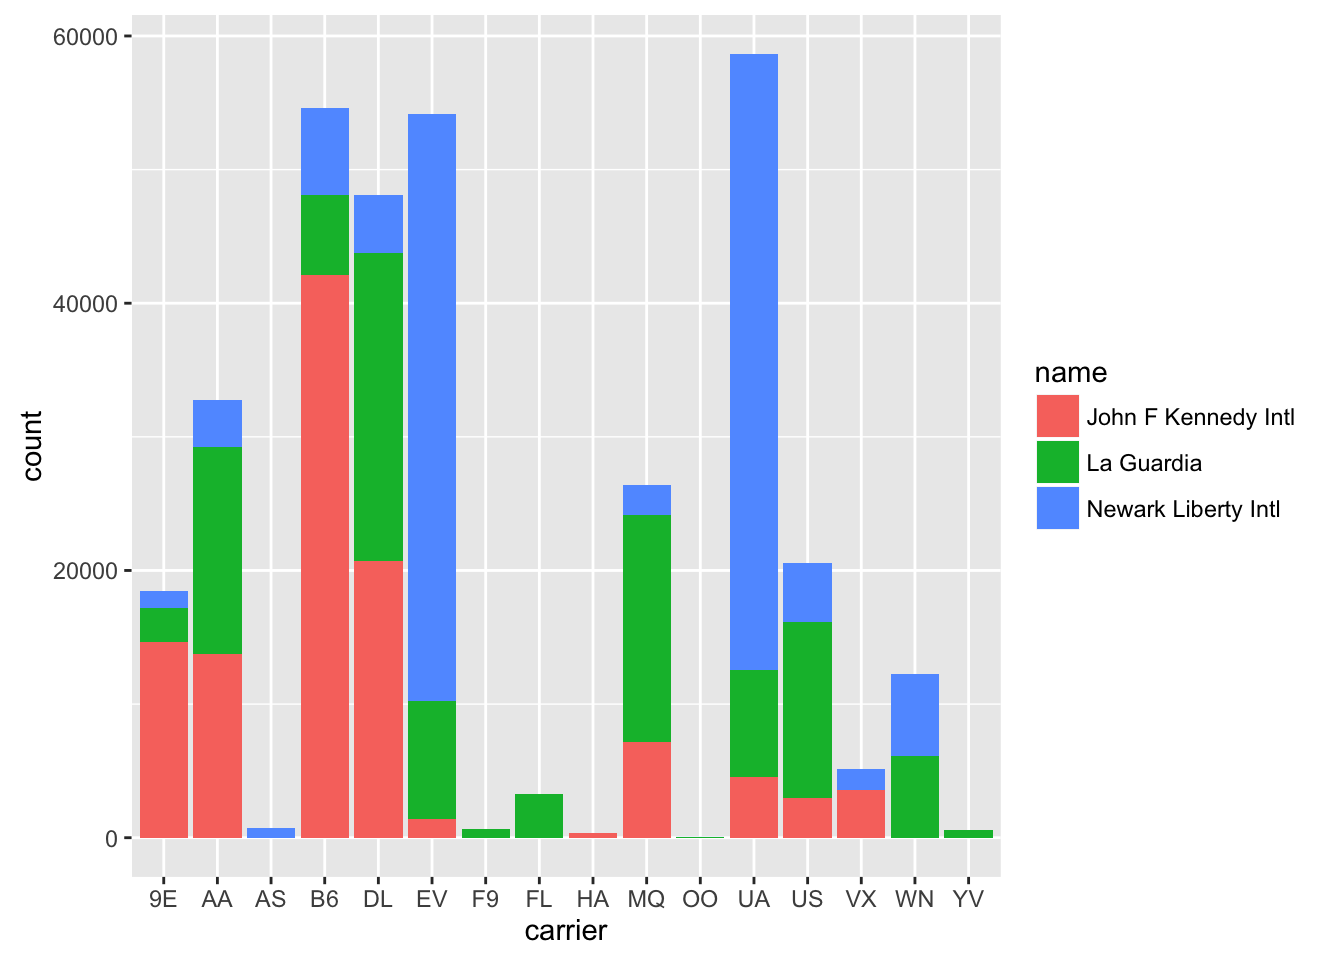
\includegraphics{ismay_kim_files/figure-latex/unnamed-chunk-27-1} \caption[Stacked barplot comparing the number of flights by carrier and airport]{Stacked barplot comparing the number of flights by carrier and airport}\label{fig:unnamed-chunk-27}
\end{figure}

This plot is what is known as a \textbf{stacked barplot}. While simple
to make, it often leads to many problems.

\begin{learncheck}
\textbf{\emph{Learning check}}
\end{learncheck}

\textbf{(LC4.19)} What kinds of questions are not easily answered by
looking at the above figure?

\textbf{(LC4.20)} What can you say, if anything, about the relationship
between airline and airport in NYC in 2013 in regards to the number of
departing flights?

\begin{center}\rule{0.5\linewidth}{\linethickness}\end{center}

Another variation on the \textbf{stacked barplot} is the
\textbf{side-by-side barplot}.

\begin{Shaded}
\begin{Highlighting}[]
\KeywordTok{ggplot}\NormalTok{(}\DataTypeTok{data =} \NormalTok{flights_namedports, }\DataTypeTok{mapping =} \KeywordTok{aes}\NormalTok{(}\DataTypeTok{x =} \NormalTok{carrier, }\DataTypeTok{fill =} \NormalTok{name)) +}
\StringTok{  }\KeywordTok{geom_bar}\NormalTok{(}\DataTypeTok{position =} \StringTok{"dodge"}\NormalTok{)}
\end{Highlighting}
\end{Shaded}

\begin{figure}
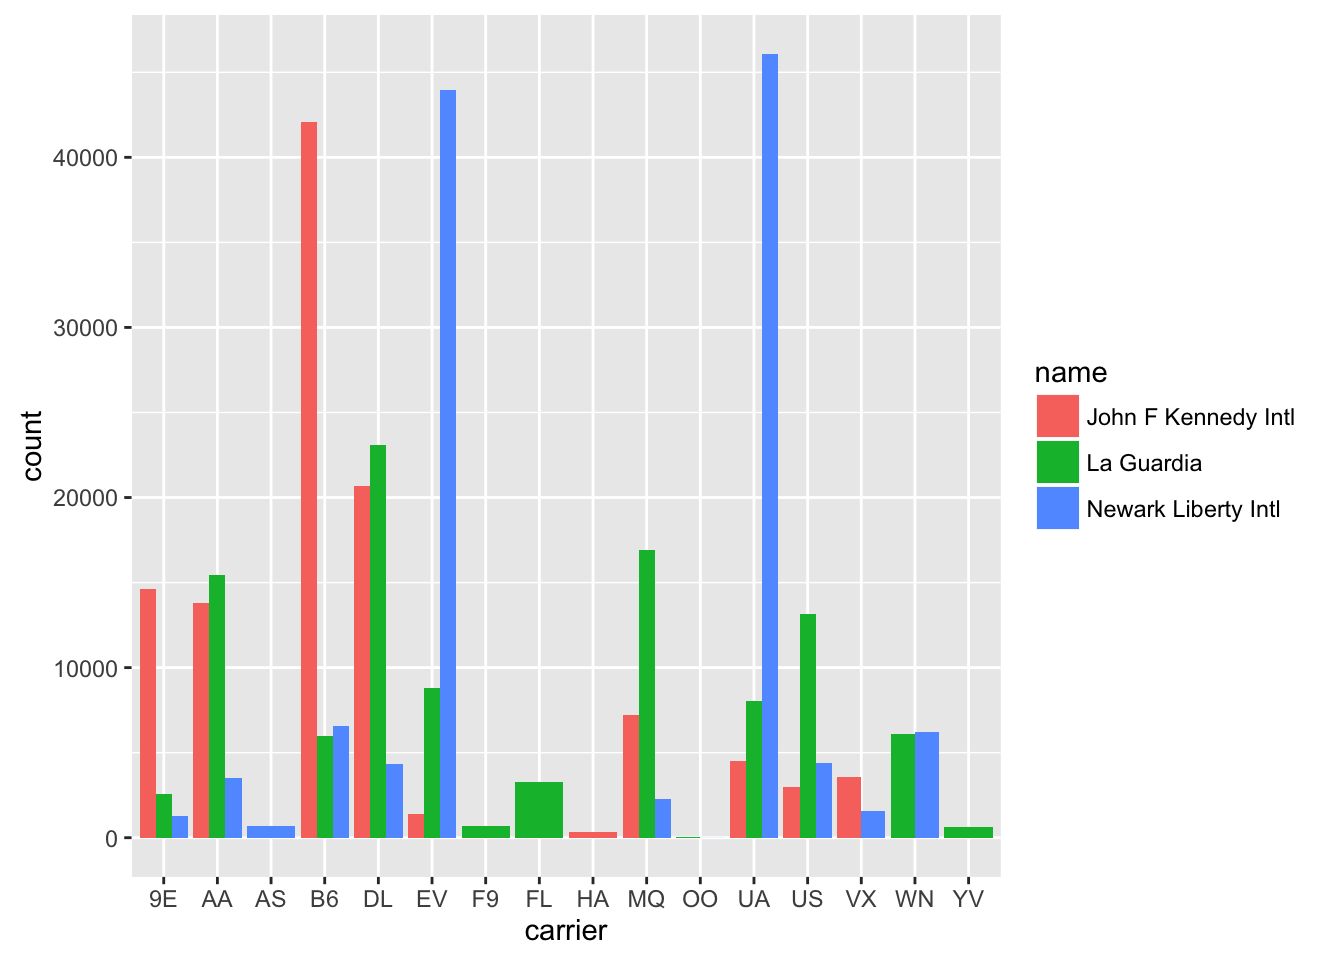
\includegraphics{ismay_kim_files/figure-latex/unnamed-chunk-28-1} \caption[Side-by-side barplot comparing the number of flights by carrier and airport]{Side-by-side barplot comparing the number of flights by carrier and airport}\label{fig:unnamed-chunk-28}
\end{figure}

\begin{center}\rule{0.5\linewidth}{\linethickness}\end{center}

\begin{learncheck}
\textbf{\emph{Learning check}}
\end{learncheck}

\textbf{(LC4.21)} Why might the side-by-side barplot be preferable to a
stacked barplot in this case?

\textbf{(LC4.22)} What are the disadvantages of using a side-by-side
barplot, in general?

\begin{center}\rule{0.5\linewidth}{\linethickness}\end{center}

Lastly, an often preferred type of barplot is the \textbf{faceted
barplot}. We already saw this concept of faceting and small multiples in
Subsection \ref{faceting}. This gives us a nicer way to compare the
distributions across both \texttt{carrier} and airport/\texttt{name}.

\begin{Shaded}
\begin{Highlighting}[]
\KeywordTok{ggplot}\NormalTok{(}\DataTypeTok{data =} \NormalTok{flights_namedports, }\DataTypeTok{mapping =} \KeywordTok{aes}\NormalTok{(}\DataTypeTok{x =} \NormalTok{carrier, }\DataTypeTok{fill =} \NormalTok{name)) +}
\StringTok{  }\KeywordTok{geom_bar}\NormalTok{() +}
\StringTok{  }\KeywordTok{facet_grid}\NormalTok{(name ~}\StringTok{ }\NormalTok{.)}
\end{Highlighting}
\end{Shaded}

\begin{figure}
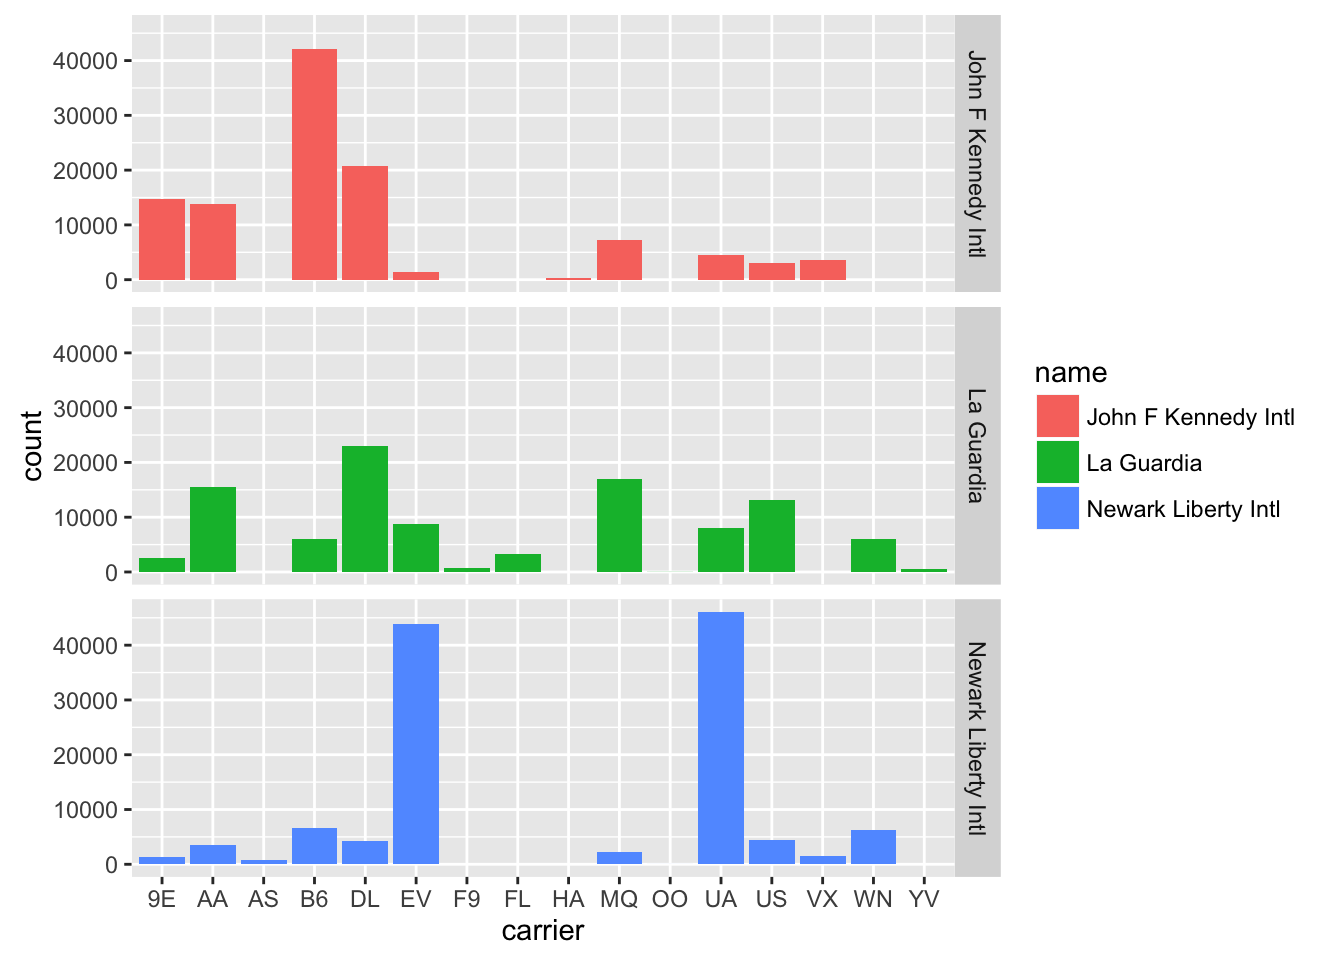
\includegraphics{ismay_kim_files/figure-latex/unnamed-chunk-29-1} \caption[Faceted barplot comparing the number of flights by carrier and airport]{Faceted barplot comparing the number of flights by carrier and airport}\label{fig:unnamed-chunk-29}
\end{figure}

Note how the \texttt{facet\_grid} function arguments are written here.
We are wanting the names of the airports vertically and the
\texttt{carrier} listed horizontally. As you may have guessed, this
argument and other \emph{formulas} of this sort in R are in
\texttt{y\ \textasciitilde{}\ x} order. We will see more examples of
this in Chapter \ref{infer}.

\begin{center}\rule{0.5\linewidth}{\linethickness}\end{center}

\begin{learncheck}
\textbf{\emph{Learning check}}
\end{learncheck}

\textbf{(LC4.23)} Why is the faceted barplot preferred to the
side-by-side and stacked barplots in this case?

\textbf{(LC4.24)} What information about the different carriers at
different airports is more easily seen in the faceted barplot?

\begin{center}\rule{0.5\linewidth}{\linethickness}\end{center}

\subsection{Summary}\label{summary-2}

Barplots are the preferred way of displaying categorical variables. They
are easy-to-understand and to make comparisons across groups of a
categorical variable. When dealing with more than one categorical
variable, faceted barplots are frequently preferred over side-by-side or
stacked barplots. Stacked barplots are sometimes nice to look at, but it
is quite difficult to compare across the levels since the sizes of the
bars are all of different sizes. Side-by-side barplots can provide an
improvement on this, but the issue about comparing across groups still
must be dealt with.

\section{Scatter-plots}\label{scatter-plots}

We have seen that boxplots are most appropriate when plotting the
distribution of ONE continuous variable across different levels/groups
of ONE categorical variable. Barplots (preferably the faceted type) are
best when looking at the distribution of ONE categorical variable across
different levels of another categorical variable. But what if we are
looking to investigate the relationship between TWO continuous
variables? What is commonly produced is the well-known
\textbf{scatter-plot}, which shows the points corresponding to the
values of each of the variables scattered around.

We will now investigate arrival delays (the vertical ``y'' axis
variable) versus departure delays (the horizontal ``x'' axis variable)
for Alaska Airlines flights leaving NYC in 2013. Notice the new function
that is invoked here: \texttt{filter}, which resides in the
\texttt{dplyr} package. You will see many more examples using this
function in Chapter \ref{manip}. The \texttt{filter} function goes
through the dataframe specified (\texttt{flights} here) and selects only
those rows which meet the condition given (\texttt{carrier\ ==\ "AS"}
here).

\begin{Shaded}
\begin{Highlighting}[]
\NormalTok{alaska_flights <-}\StringTok{ }\KeywordTok{filter}\NormalTok{(flights, carrier ==}\StringTok{ "AS"}\NormalTok{)}
\KeywordTok{ggplot}\NormalTok{(alaska_flights, }\KeywordTok{aes}\NormalTok{(}\DataTypeTok{x =} \NormalTok{dep_delay, }\DataTypeTok{y =} \NormalTok{arr_delay)) +}\StringTok{ }
\StringTok{  }\KeywordTok{geom_point}\NormalTok{()}
\end{Highlighting}
\end{Shaded}

\begin{figure}
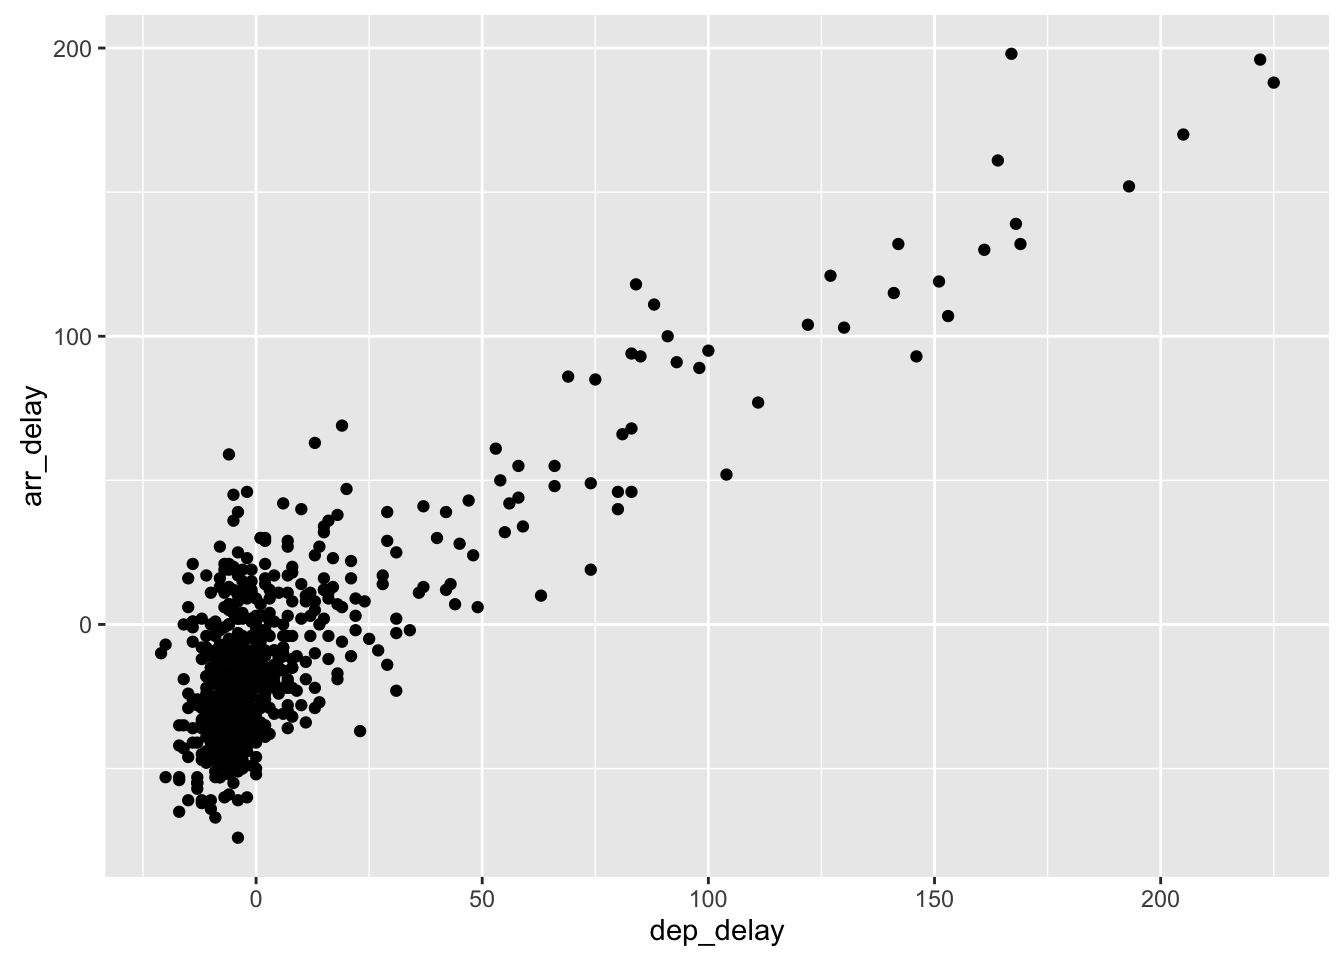
\includegraphics{ismay_kim_files/figure-latex/noalpha-1} \caption[Arrival Delays vs Departure Delays for Alaska Airlines flights from NYC in 2013]{Arrival Delays vs Departure Delays for Alaska Airlines flights from NYC in 2013}\label{fig:noalpha}
\end{figure}

We see that a positive relationship exists between \texttt{dep\_delay}
and \texttt{arr\_delay}: as departure delays increase, arrival delays
tend to also increase. We also note that the majority of points fall
near the point (0, 0) here. There is a large mass of points clustered
there.

\begin{center}\rule{0.5\linewidth}{\linethickness}\end{center}

\begin{learncheck}
\textbf{\emph{Learning check}}
\end{learncheck}

\textbf{(LC4.25)} What are some practical reasons why
\texttt{dep\_delay} and \texttt{arr\_delay} have a positive
relationship?

\textbf{(LC4.26)} What variables (not necessarily in the
\texttt{flights} dataframe) would you expect to have a negative
correlation (i.e.~a negative relationship) with \texttt{dep\_delay}?
Why? Remember that we are focusing on continuous variables here.

\textbf{(LC4.27)} Why do you believe there is a cluster of points near
(0, 0)?

\begin{itemize}
\tightlist
\item
  What does (0, 0) correspond to in terms of the Alaskan flights?
\end{itemize}

\textbf{(LC4.28)} What are some other features of the plot that stand
out to you?

\begin{center}\rule{0.5\linewidth}{\linethickness}\end{center}

\subsection{Jittering}\label{jittering}

The large mass of points near (0, 0) can cause some confusion. This is
the result of a phenomenon called \textbf{over-plotting}. As one may
guess, this corresponds to values being plotted on top of each other
\emph{over} and \emph{over} again. It is often difficult to know just
how many values are plotted in this way when looking at a basic
scatter-plot as we have here.

One way of relieving this issue of \textbf{over-plotting} is to
\textbf{jitter} the points a bit. In other words, we are going to add
just a bit of random noise to the points to better see them and remove
some of the over-plotting. You can think of ``jittering'' as shaking the
points a bit on the plot. Instead of using \texttt{geom\_point}, we use
\texttt{geom\_jitter} to perform this shaking and specify around how
much jitter to add with the \texttt{width} and \texttt{height}
arguments. This corresponds to how hard you'd like to shake the plot in
units corresponding to those for both the horizontal and vertical
variables (minutes here).

\begin{Shaded}
\begin{Highlighting}[]
\KeywordTok{ggplot}\NormalTok{(alaska_flights, }\KeywordTok{aes}\NormalTok{(}\DataTypeTok{x =} \NormalTok{dep_delay, }\DataTypeTok{y =} \NormalTok{arr_delay)) +}\StringTok{ }
\StringTok{  }\KeywordTok{geom_jitter}\NormalTok{(}\DataTypeTok{width =} \DecValTok{30}\NormalTok{, }\DataTypeTok{height =} \DecValTok{30}\NormalTok{)}
\end{Highlighting}
\end{Shaded}

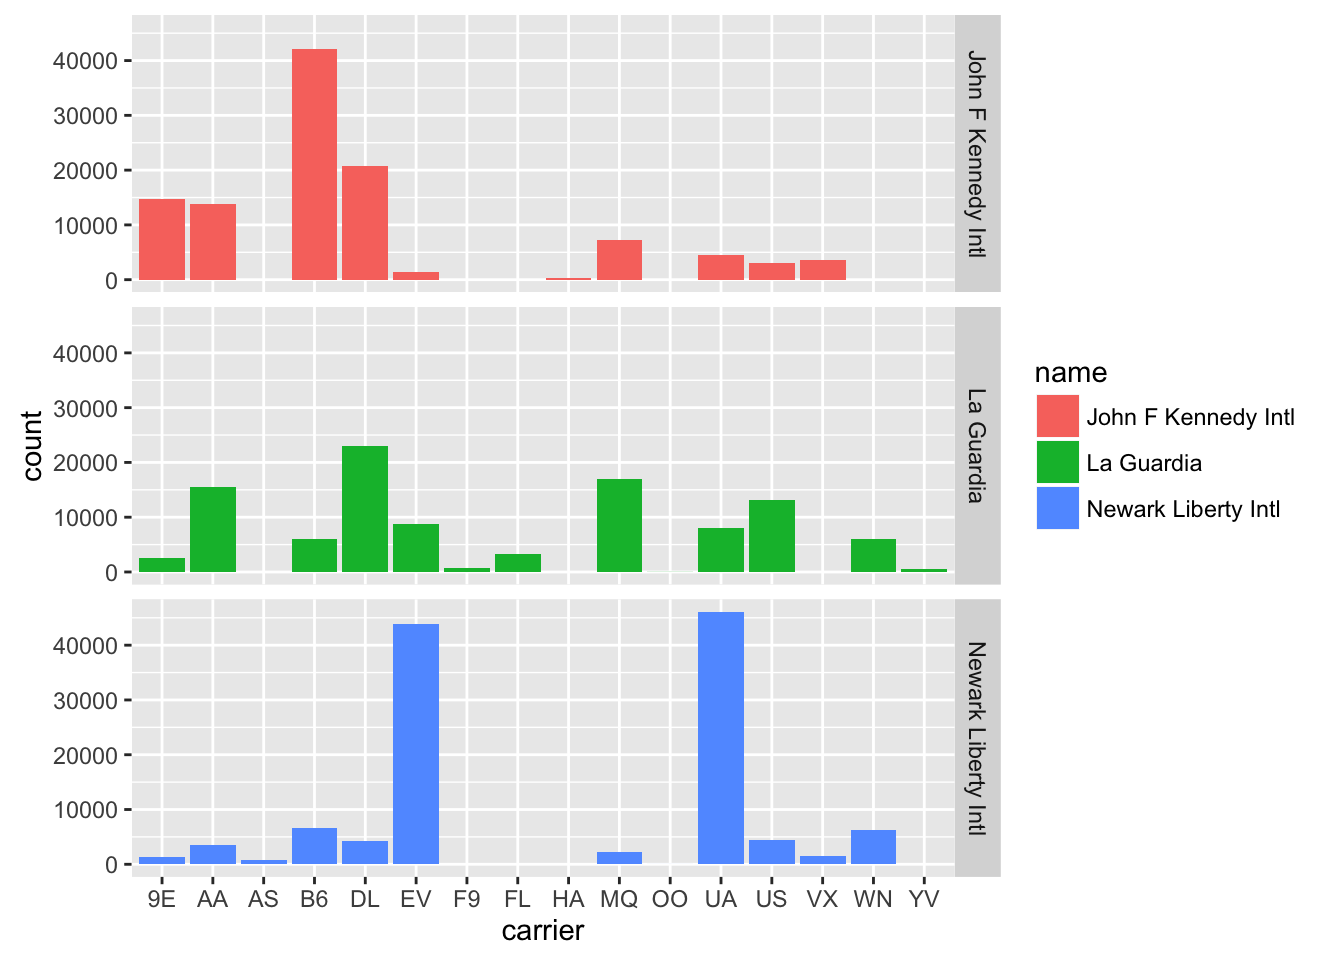
\includegraphics{ismay_kim_files/figure-latex/unnamed-chunk-31-1}

This has helps us a little bit in getting a sense for the over-plotting,
but with a relatively large dataset like this one (714 flights), it is
often useful to change the transparency of the points as seen in the
next section.

\subsection{Setting transparency}\label{setting-transparency}

One of the arguments that can be changed with \texttt{geom\_point} is
\texttt{alpha}. By default, this value is set to \texttt{1}. We can
change this value to a smaller fraction to change the transparency of
the points in the plot:

\begin{Shaded}
\begin{Highlighting}[]
\KeywordTok{ggplot}\NormalTok{(alaska_flights, }\KeywordTok{aes}\NormalTok{(}\DataTypeTok{x =} \NormalTok{dep_delay, }\DataTypeTok{y =} \NormalTok{arr_delay)) +}\StringTok{ }
\StringTok{  }\KeywordTok{geom_point}\NormalTok{(}\DataTypeTok{alpha =} \FloatTok{0.2}\NormalTok{)}
\end{Highlighting}
\end{Shaded}

\begin{figure}
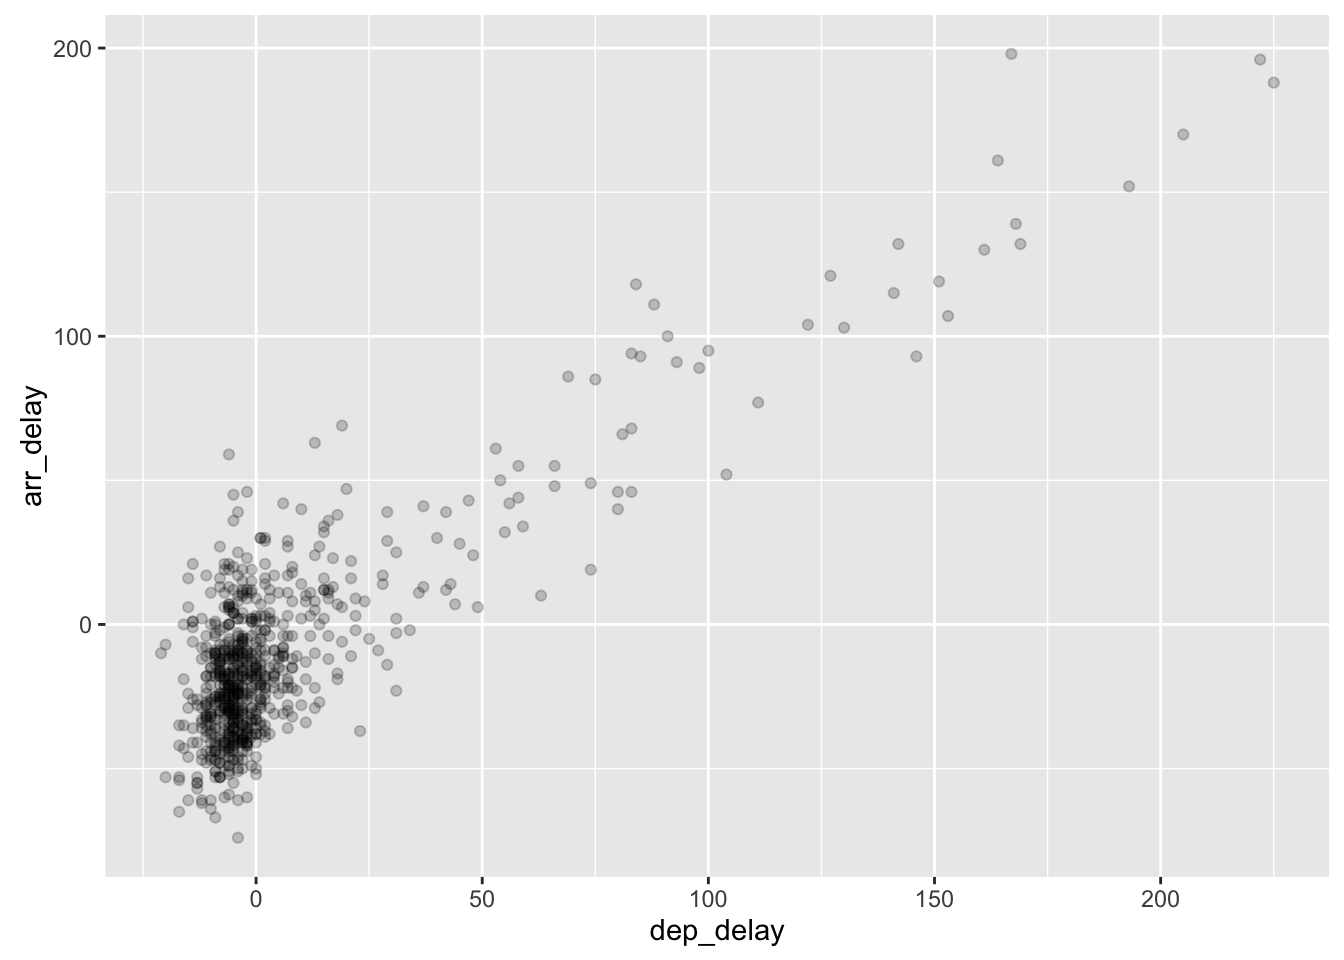
\includegraphics{ismay_kim_files/figure-latex/alpha-1} \caption[Arrival Delays vs Departure Delays for Alaska Airlines flights from NYC in 2013 - alpha=0]{Arrival Delays vs Departure Delays for Alaska Airlines flights from NYC in 2013 - alpha=0.2}\label{fig:alpha}
\end{figure}

We can also specify the \texttt{alpha} argument in
\texttt{geom\_jitter}:

\begin{Shaded}
\begin{Highlighting}[]
\KeywordTok{ggplot}\NormalTok{(alaska_flights, }\KeywordTok{aes}\NormalTok{(}\DataTypeTok{x =} \NormalTok{dep_delay, }\DataTypeTok{y =} \NormalTok{arr_delay)) +}\StringTok{ }
\StringTok{  }\KeywordTok{geom_jitter}\NormalTok{(}\DataTypeTok{width =} \DecValTok{30}\NormalTok{, }\DataTypeTok{height =} \DecValTok{30}\NormalTok{, }\DataTypeTok{alpha =} \FloatTok{0.3}\NormalTok{)}
\end{Highlighting}
\end{Shaded}

\begin{figure}
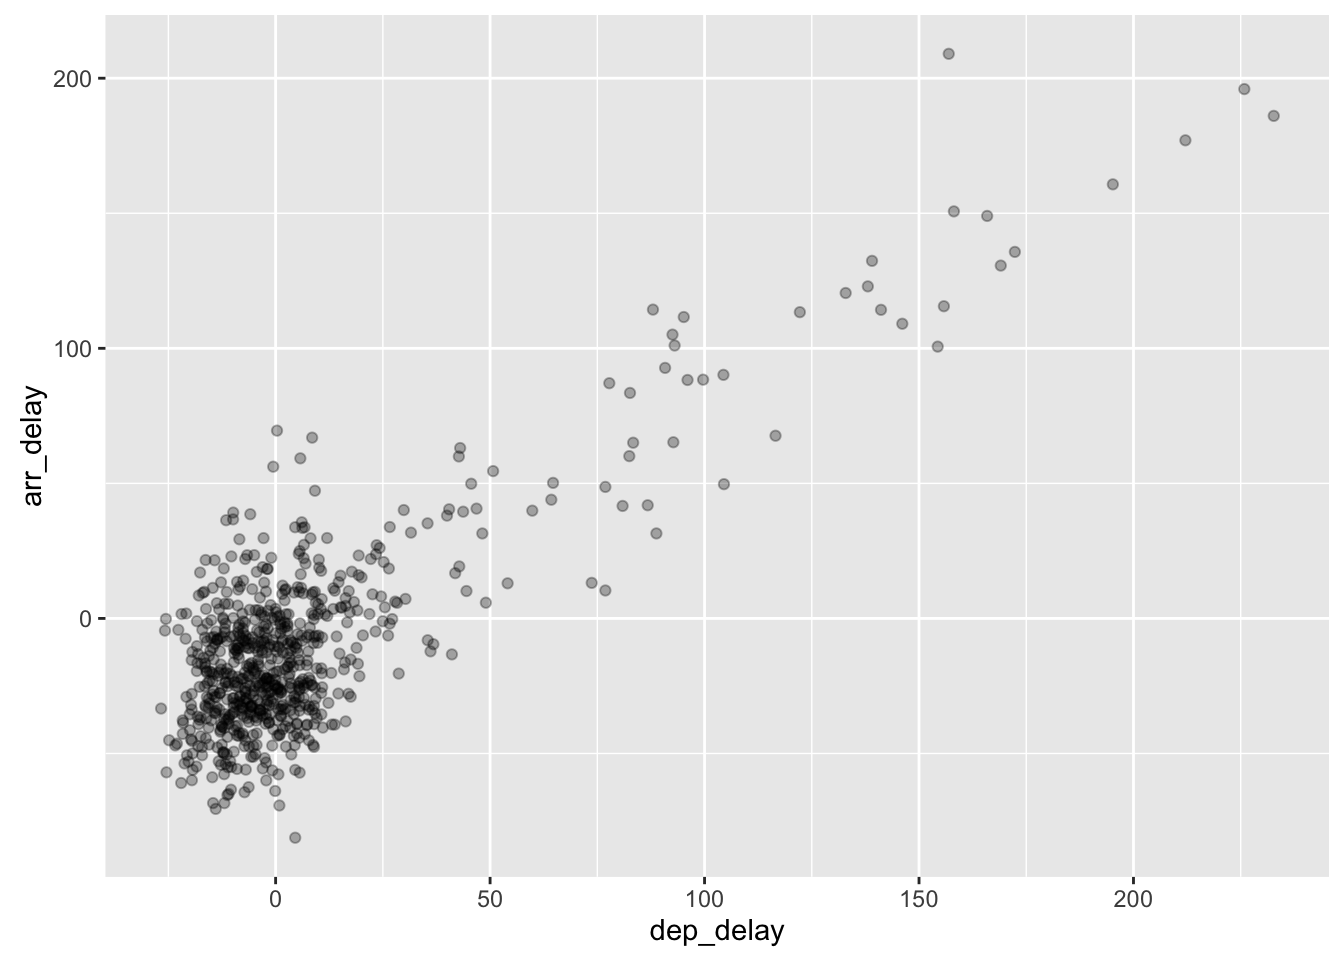
\includegraphics{ismay_kim_files/figure-latex/jitteralpha-1} \caption[Arrival Delays vs Departure Delays for Alaska Airlines flights from NYC in 2013 - jitter and alpha added]{Arrival Delays vs Departure Delays for Alaska Airlines flights from NYC in 2013 - jitter and alpha added}\label{fig:jitteralpha}
\end{figure}

\begin{center}\rule{0.5\linewidth}{\linethickness}\end{center}

\begin{learncheck}
\textbf{\emph{Learning check}}
\end{learncheck}

\textbf{(LC4.29)} Why is setting the \texttt{alpha} argument value
useful with scatter-plots?

\begin{itemize}
\tightlist
\item
  What further information does it give you that a regular scatter-plot
  cannot?
\end{itemize}

\textbf{(LC4.30)} After viewing the \ref{fig:alpha} above, give a range
of arrival times and departure times that occur most frequently?

\begin{itemize}
\tightlist
\item
  How has that region changed compared to when you observed the same
  plot without the \texttt{alpha\ =\ 0.2} set in \ref{fig:noalpha}?
\end{itemize}

\begin{center}\rule{0.5\linewidth}{\linethickness}\end{center}

\textbf{Maybe include a shading of the points by another variable
example here for multivariate thinking?}

\subsection{Summary}\label{summary-3}

Scatter-plots may be the most used plot today and they can provide an
immediate way to see the trend in one variable versus another. Remember
that they only make sense when plotting a continuous variable versus a
continuous variable though. If you try to create a scatter-plot where
either one of the two variables is not quantitative, you will get
strange results. Be careful!

With medium to large datasets, you may need to tweak arguments in both
\texttt{geom\_jitter} and the \texttt{alpha} parameter in order to get a
good feel for relationships in your data. This tweaking is often a fun
part of data visualization since you'll have the chance to see different
relationships come about as you make subtle changes to your plots.

\section{Line-graphs}\label{line-graphs}

The last of the FNG is a line-graph. They are most frequently used when
the horizontal axis is time. Time represents a variable that is
connected together by each day following the previous day. In other
words, time has a natural ordering. Line-graphs should be avoided when
there is not a clear ordering to the explanatory (``x'' variable).

We are interested in exploring the arrival delays by day throughout the
year of 2013 from outgoing flights from New York City. If we plotted all
of these values, we obtain the following scatter-plot:

\begin{Shaded}
\begin{Highlighting}[]
\KeywordTok{ggplot}\NormalTok{(flights, }\KeywordTok{aes}\NormalTok{(}\DataTypeTok{x =} \NormalTok{time_hour, }\DataTypeTok{y =} \NormalTok{arr_delay)) +}\StringTok{ }
\StringTok{  }\KeywordTok{geom_point}\NormalTok{()}
\end{Highlighting}
\end{Shaded}

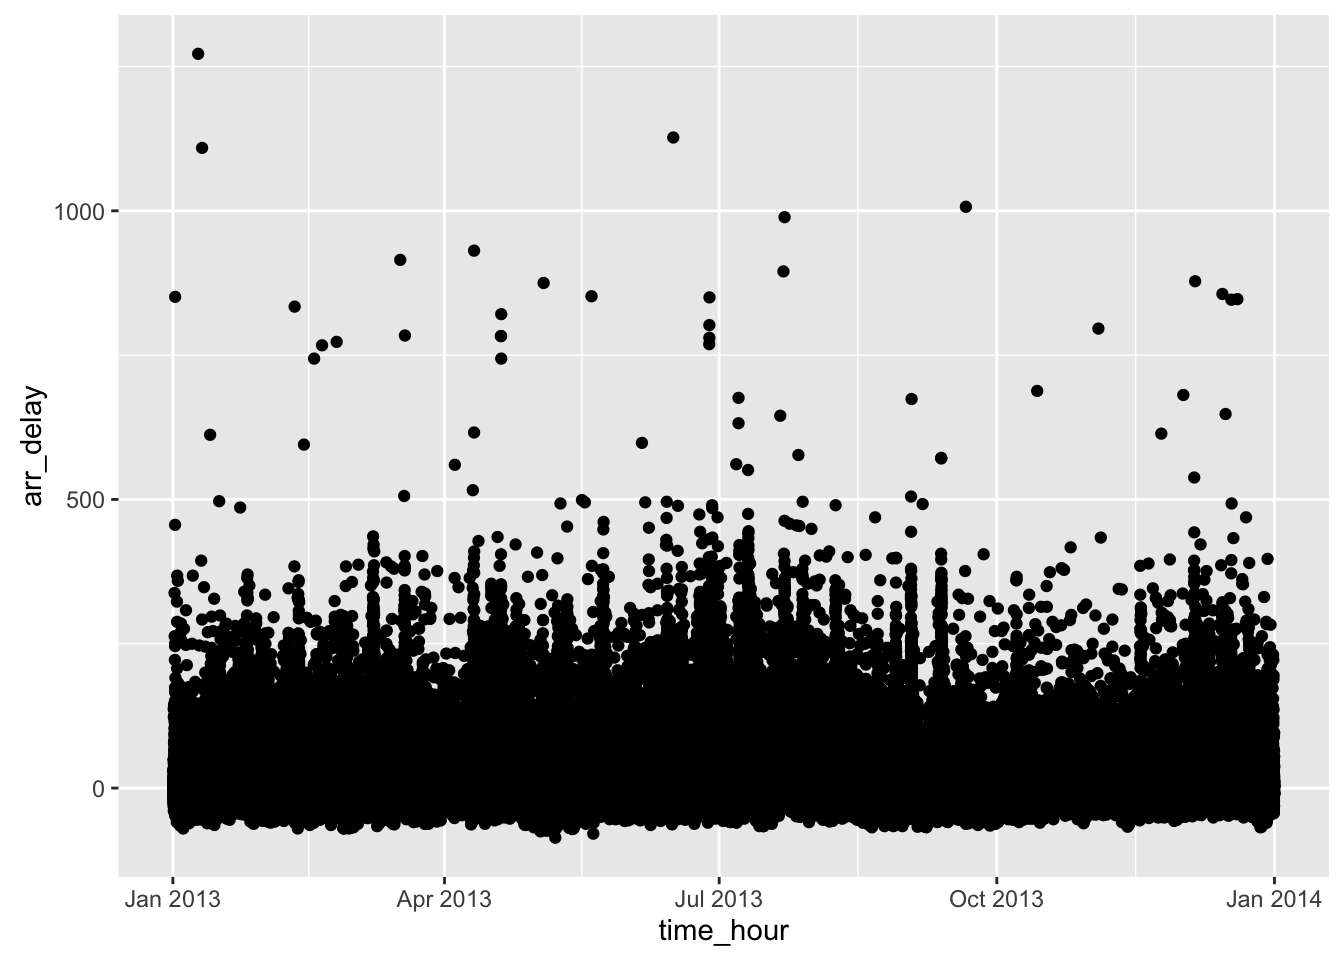
\includegraphics{ismay_kim_files/figure-latex/unnamed-chunk-32-1}

We see that this plot is difficult to understand based on the sheer
number of points plotted. We see some outlier points with more than 500
minutes of arrival delay, but even some jittering and transparency is
not going to help us here.

Instead of plotting all of the values for each hour for all flights, it
might make sense to plot the average value for each day in terms of
arrival delays. Of course, we also need to address which average we
should use: mean or median. With there being some outliers here, we have
chosen to use the median arrival delay (since the mean is heavily
influence by outliers).

You may think that this is a difficult task but the \texttt{group\_by}
and \texttt{summarize} functions make this a breeze. You'll see more
examples using these two functions in Chapter \ref{manip}. Here we will
create a new variable, which corresponds to the month and day combined,
from the \texttt{time\_hour} column using the \texttt{mutate} function
and create a new dataframe called \texttt{flights\_day}. We also give
the \texttt{str} of this new dataset so you can see the new variable
added \texttt{date}:

\begin{Shaded}
\begin{Highlighting}[]
\NormalTok{flights_day <-}\StringTok{ }\KeywordTok{mutate}\NormalTok{(flights, }\DataTypeTok{date =} \KeywordTok{as.Date}\NormalTok{(time_hour))}
\KeywordTok{str}\NormalTok{(flights_day)}
\end{Highlighting}
\end{Shaded}

\begin{verbatim}
## Classes 'tbl_df', 'tbl' and 'data.frame':    336776 obs. of  20 variables:
##  $ year          : int  2013 2013 2013 2013 2013 2013 2013 2013 2013 2013 ...
##  $ month         : int  1 1 1 1 1 1 1 1 1 1 ...
##  $ day           : int  1 1 1 1 1 1 1 1 1 1 ...
##  $ dep_time      : int  517 533 542 544 554 554 555 557 557 558 ...
##  $ sched_dep_time: int  515 529 540 545 600 558 600 600 600 600 ...
##  $ dep_delay     : num  2 4 2 -1 -6 -4 -5 -3 -3 -2 ...
##  $ arr_time      : int  830 850 923 1004 812 740 913 709 838 753 ...
##  $ sched_arr_time: int  819 830 850 1022 837 728 854 723 846 745 ...
##  $ arr_delay     : num  11 20 33 -18 -25 12 19 -14 -8 8 ...
##  $ carrier       : chr  "UA" "UA" "AA" "B6" ...
##  $ flight        : int  1545 1714 1141 725 461 1696 507 5708 79 301 ...
##  $ tailnum       : chr  "N14228" "N24211" "N619AA" "N804JB" ...
##  $ origin        : chr  "EWR" "LGA" "JFK" "JFK" ...
##  $ dest          : chr  "IAH" "IAH" "MIA" "BQN" ...
##  $ air_time      : num  227 227 160 183 116 150 158 53 140 138 ...
##  $ distance      : num  1400 1416 1089 1576 762 ...
##  $ hour          : num  5 5 5 5 6 5 6 6 6 6 ...
##  $ minute        : num  15 29 40 45 0 58 0 0 0 0 ...
##  $ time_hour     : POSIXct, format: "2013-01-01 05:00:00" ...
##  $ date          : Date, format: "2013-01-01" ...
\end{verbatim}

\begin{Shaded}
\begin{Highlighting}[]
\NormalTok{flights_summarized <-}\StringTok{ }\NormalTok{flights_day %>%}\StringTok{ }\KeywordTok{group_by}\NormalTok{(date) %>%}
\StringTok{  }\KeywordTok{summarize}\NormalTok{(}\DataTypeTok{median_arr_delay =} \KeywordTok{median}\NormalTok{(arr_delay, }\DataTypeTok{na.rm =} \OtherTok{TRUE}\NormalTok{))}
\KeywordTok{head}\NormalTok{(flights_summarized)}
\end{Highlighting}
\end{Shaded}

\begin{verbatim}
## # A tibble: 6 x 2
##         date median_arr_delay
##       <date>            <dbl>
## 1 2013-01-01                3
## 2 2013-01-02                4
## 3 2013-01-03                1
## 4 2013-01-04               -8
## 5 2013-01-05               -7
## 6 2013-01-06               -1
\end{verbatim}

You will see the ``pipe'' operator \texttt{\%\textgreater{}\%} explained
in more detail in Chapter \ref{manip}, but you can read it as ``and
then''. Here, we take the \texttt{flights\_day} dataframe that we just
created and then group it together by \texttt{date}. This goes through
the dataframe and puts together all rows that have \texttt{2013-01-01}
together, all rows that have \texttt{2013-01-02} together, \ldots{}, and
all rows that have \texttt{2013-12-31} together. And then it looks at
the median value of \texttt{arr\_delay} over each one of the days. You
can get a glimpse of the first few rows of this new dataset above since
we invoked the \texttt{head} function on it.

Note also that there are missing values in this data set so we need to
exclude them from the analysis. This is why the \texttt{na.rm\ =\ TRUE}
argument is invoked. Many functions require this extra specification so
it's always a good idea to run a \texttt{?median} or \texttt{?mean}
before you try to run the function. Or you can always run it afterwards
as well when you get strange results.

Now getting back to our line-graph. We want to plot the median arrival
delay over all airlines on all days in 2013 from departing flights in
NYC. This syntax should look similar to what we have seen before with
plots involving \texttt{ggplot}. Notice that we are using the
\texttt{flights\_summarized} dataset here and not the
\texttt{flights\_day} or \texttt{flights} dataframes.

\begin{Shaded}
\begin{Highlighting}[]
\KeywordTok{ggplot}\NormalTok{(}\DataTypeTok{data =} \NormalTok{flights_summarized, }\KeywordTok{aes}\NormalTok{(}\DataTypeTok{x =} \NormalTok{date, }\DataTypeTok{y =} \NormalTok{median_arr_delay)) +}
\StringTok{  }\KeywordTok{geom_line}\NormalTok{()}
\end{Highlighting}
\end{Shaded}

\begin{figure}
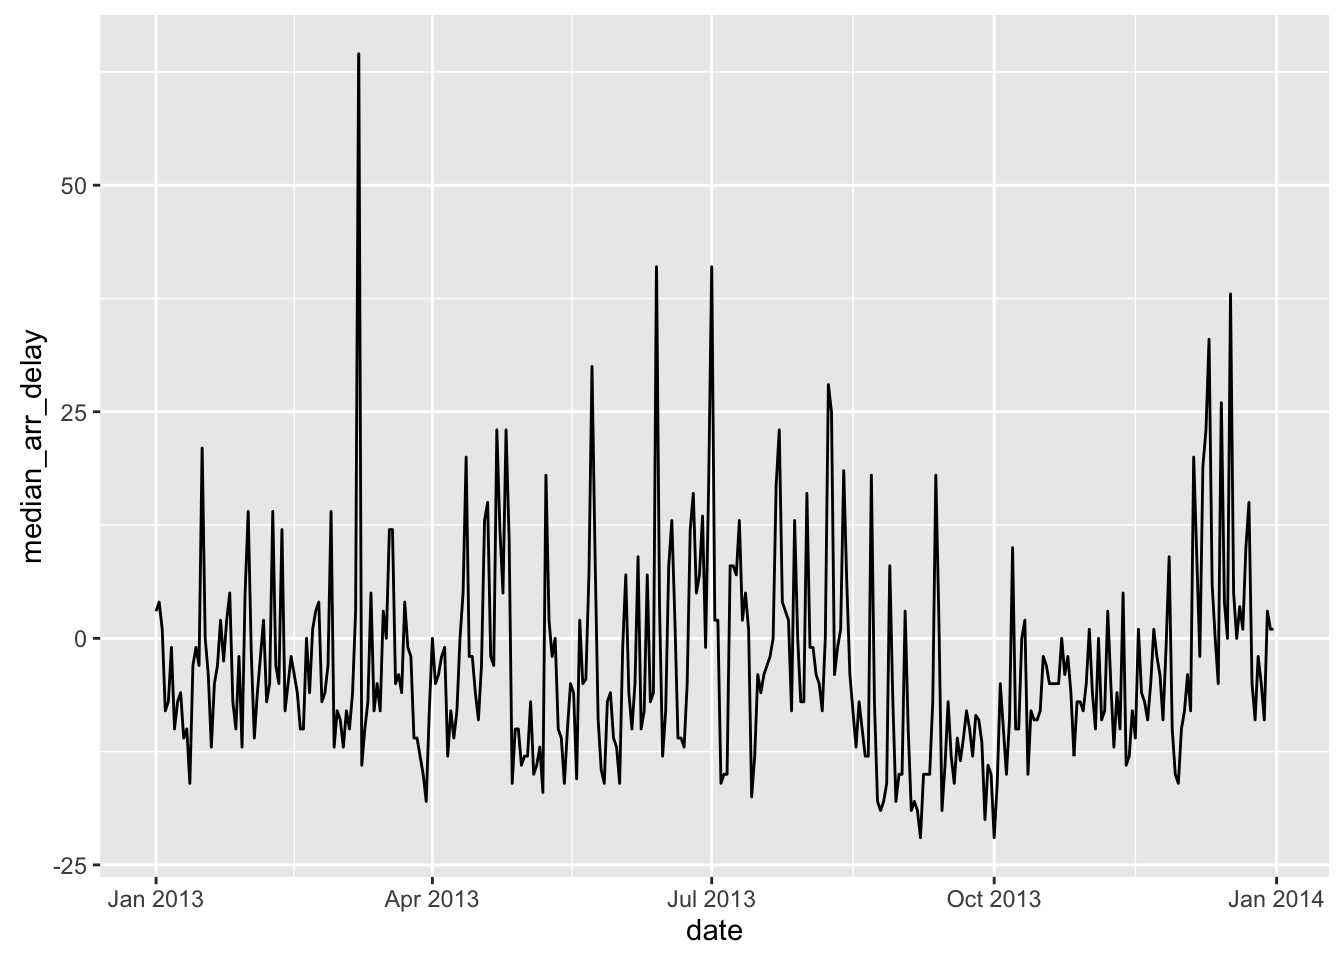
\includegraphics{ismay_kim_files/figure-latex/lineflights-1} \caption[Line-graph of median arrival delay for flights leaving NYC in 2013 versus day of the year]{Line-graph of median arrival delay for flights leaving NYC in 2013 versus day of the year}\label{fig:lineflights}
\end{figure}

\subsection{Interactive line-graphs}\label{interactive-line-graphs}

Another useful tool for viewing line-graphs such as this is the
\texttt{dygraph} function in the \texttt{dygraphs} package in
combination with the \texttt{dyRangeSelector} function. This allows us
to zoom in on a selected range and get an interactive plot for us to
work with:

\begin{Shaded}
\begin{Highlighting}[]
\KeywordTok{library}\NormalTok{(dygraphs)}
\KeywordTok{rownames}\NormalTok{(flights_summarized) <-}\StringTok{ }\NormalTok{flights_summarized$date}
\NormalTok{flights_summarized <-}\StringTok{ }\KeywordTok{select}\NormalTok{(flights_summarized, -date)}
\KeywordTok{dyRangeSelector}\NormalTok{(}\KeywordTok{dygraph}\NormalTok{(flights_summarized))}
\end{Highlighting}
\end{Shaded}

\includegraphics{ismay_kim_files/figure-latex/unnamed-chunk-35-1}

The syntax here is a little different than what we have covered so far.
The \texttt{dygraph} function is expecting for the dates to be given as
the \texttt{rownames} of the object. We then remove the \texttt{date}
variable from the \texttt{flights\_summarized} dataframe since it is
accounted for in the \texttt{rownames}. Lastly, we run the
\texttt{dygraph} function on the new dataframe that only contains the
median arrival delay as a column and then provide the ability to have a
selector to zoom in on the interactive plot via
\texttt{dyRangeSelector}. (Note that this plot will only be interactive
in the HTML version of this book.)

\textbf{Include this interactive dygraphs stuff here or in Appendix B?}

\textbf{Include bad example of when a line-graph would be invalid?}

\begin{center}\rule{0.5\linewidth}{\linethickness}\end{center}

\begin{learncheck}
\textbf{\emph{Learning check}}
\end{learncheck}

\textbf{(LC4.31)} Why should line-graphs be avoided when there is not a
clear ordering of the horizontal axis?

\textbf{(LC4.32)} Why are line-graphs frequently used when time is the
explanatory variable?

\textbf{(LC4.33)} Why did we use the \texttt{flights\_summarized}
dataframe to produce the line-graph in Figure \ref{fig:lineflights}
instead of \texttt{flights} or \texttt{flights\_day}?

\textbf{(LC4.34)} Are the largest median arrival delays where you
expected them to occur on the line-graph above in Figure
\ref{lineflights}?

\textbf{(LC4.35)} Use the interactive line-graph to determine the
highest median arrival delay for flights from NYC in 2013. What date was
it and what do you think contributed to it?

\begin{center}\rule{0.5\linewidth}{\linethickness}\end{center}

\subsection{Summary}\label{summary-4}

Line-graphs provide a useful tool for viewing a continuous variable that
is plotted versus time. We need to be careful to not be too entrenched
in using line-graphs whenever we wish though. They only make sense when
the explanatory variable (the one on the explanatory variable) has a
natural ordering. We can mislead our audience if that isn't the case.

\section{Brief Review of The Grammar of
Graphics}\label{brief-review-of-the-grammar-of-graphics}

You have seen all of the major pieces behind ``The Grammar of Graphics''
which serves as the basis for the \texttt{ggplot2} package. Here is a
summary of each part:

\textbf{May need some tweaking}:
\url{http://www.ling.upenn.edu/~joseff/avml2012/}

\begin{center}\rule{0.5\linewidth}{\linethickness}\end{center}

\begin{center}\rule{0.5\linewidth}{\linethickness}\end{center}

\begin{review}
\textbf{\emph{Review questions}}
\end{review}

\textbf{(RQ4.1)}

\begin{itemize}
\item
  Have a variety of bad plots with data for the readers and have readers
  create better plots with \texttt{ggplot2}
\item
  Have sample datasets to work with from problem statements

  \begin{itemize}
  \tightlist
  \item
    Identify the appropriate plot to address the questions of interest
  \end{itemize}
\item
  Why is it important for barplots to start at zero?
\end{itemize}

\begin{center}\rule{0.5\linewidth}{\linethickness}\end{center}

\begin{center}\rule{0.5\linewidth}{\linethickness}\end{center}

\section{What's to come?}\label{whats-to-come-1}

\textbf{Last updated:}

\begin{verbatim}
## [1] "Tuesday, August 02, 2016 13:47:57 CDT"
\end{verbatim}

\chapter{Manipulating Data}\label{manip}

\begin{itemize}
\tightlist
\item
  Going through a lot of examples with \texttt{dplyr} here

  \begin{itemize}
  \tightlist
  \item
    Definitely want to introduce them to the pipe
  \item
    Show why it is so much better than nesting/temporary variables
  \item
    Show how to get the summary statistics mentioned in Viz across
    groups with \texttt{group\_by} and \texttt{summarize}
  \item
    Show how to rename variables such as the \texttt{name} column from
    \texttt{airlines}
  \item
    Get number of elements in specific columns similar to
    \texttt{table()} function with \texttt{dplyr}
  \item
    \href{https://github.com/Amherst-Statistics}{Nick Horton's slides
    from JSM}
  \end{itemize}
\item
  Database normalization
\item
  \url{https://en.wikipedia.org/wiki/Database_normalization}
\item
  Add importance of joining tables
\item
  Make sure to refer back to plots in the viz chapter and how the
  material here relates to answering those questions
\item
  We'll also need to address how this leads into inference
\end{itemize}

\chapter{Collecting Data}\label{collect}

More traditional in feel

\begin{itemize}
\tightlist
\item
  (random) Sampling: representativeness/generalizability/bias
\item
  Observational study vs randomized experiment (fit with correlation)
\item
  Confounding variables
\end{itemize}

\chapter{Inference}\label{infer}

\begin{itemize}
\tightlist
\item
  Standard errors and sampling distribution via randomization

  \begin{itemize}
  \tightlist
  \item
    Developing traditional inference from randomization
  \item
    two-sample permutation test -\textgreater{} null distribution\\
  \item
    Showing what happens when assumptions/conditions aren't met
  \item
    Then show normal/t-test and show how it fits on top of sampling
    distribution
  \end{itemize}
\item
  Hypothesis testing

  \begin{itemize}
  \tightlist
  \item
    The theory of hypothesis. Criminal justice. Question: what do you do
    with a problem like alpha?
  \end{itemize}
\item
  Confidence intervals
\item
  Simple linear regression
\item
  Multiple regression

  \begin{itemize}
  \tightlist
  \item
    Regression/correlation/multiple regression/confounding
  \item
    Categorical predictor and baseline
  \item
    Implement \texttt{tidy}, \texttt{broom::augment}, and
    \texttt{glance} in \texttt{broom} package to get results
  \item
    Model selection is a can of worms
  \item
    Cross-validation

    \begin{itemize}
    \tightlist
    \item
      Take half of dataset for fit, use to predict other half.

      \begin{itemize}
      \tightlist
      \item
        Show random sampling of half matters
      \item
        Is only once enough?
      \end{itemize}
    \end{itemize}
  \end{itemize}
\end{itemize}

\section{Topics to be Dropped}\label{topics-to-be-dropped}

\begin{itemize}
\tightlist
\item
  Design of experiments
\item
  statistical power
\item
  Independence/Probability
\item
  Chi-Square Tests
\item
  Not do extensive ANOVA, but allude to it after doing multiple
  regression with categorical
\item
  Logistic Regression
\item
  CLT/Mathematical computation engine (but we need to ascertain the
  unintended consequences of dropping it)

  \begin{itemize}
  \tightlist
  \item
    Tell them the minimum they need to know
  \end{itemize}
\end{itemize}

\chapter{Appendix A: R and RStudio Basics}\label{appendix1}

\begin{itemize}
\tightlist
\item
  What is R? What is RStudio?
\item
  Screenshots of RStudio frames?
\item
  Installing R and RStudio directions with screenshots
\item
  Give an introduction into using R
\item
  Mean, median, standard deviation, five-number summary, distribution
\item
  Some content to cover:

  \begin{itemize}
  \tightlist
  \item
    data structures (vectors, lists, data frames, matrices)
  \item
    indexing/subsetting
  \item
    functions (default arguments)
  \item
    Case matters in R!
  \item
    Why do some arguments require quotations and others don't?
  \end{itemize}
\item
  RMarkdown chunk options
\item
  Help -\textgreater{} Cheatsheets
\end{itemize}

\chapter{Appendix B: Intermediate R}\label{appendix2}

\section{Sorted barplots}\label{sorted-barplots}

Building upon the example in Section \ref{barplots}:

\begin{Shaded}
\begin{Highlighting}[]
\KeywordTok{library}\NormalTok{(nycflights13)}
\KeywordTok{library}\NormalTok{(ggplot2)}
\NormalTok{flights_table <-}\StringTok{ }\KeywordTok{table}\NormalTok{(flights$carrier)}
\NormalTok{flights_table}
\end{Highlighting}
\end{Shaded}

\begin{verbatim}
## 
##    9E    AA    AS    B6    DL    EV    F9    FL    HA    MQ    OO    UA 
## 18460 32729   714 54635 48110 54173   685  3260   342 26397    32 58665 
##    US    VX    WN    YV 
## 20536  5162 12275   601
\end{verbatim}

\begin{Shaded}
\begin{Highlighting}[]
\CommentTok{#library(dplyr)}
\CommentTok{#carrier_counts <- flights %>% count(carrier)}
\CommentTok{#carrier_counts}
\end{Highlighting}
\end{Shaded}

We can sort this table from highest to lowest counts by using the
\texttt{sort} function:

\begin{Shaded}
\begin{Highlighting}[]
\NormalTok{sorted_flights <-}\StringTok{ }\KeywordTok{sort}\NormalTok{(flights_table, }\DataTypeTok{decreasing =} \OtherTok{TRUE}\NormalTok{)}
\KeywordTok{names}\NormalTok{(sorted_flights)}
\end{Highlighting}
\end{Shaded}

\begin{verbatim}
##  [1] "UA" "B6" "EV" "DL" "AA" "MQ" "US" "9E" "WN" "VX" "FL" "AS" "F9"
## [14] "YV" "HA" "OO"
\end{verbatim}

\begin{Shaded}
\begin{Highlighting}[]
\CommentTok{#carrier_counts <- carrier_counts %>%}
\CommentTok{#  arrange(desc(n))}
\end{Highlighting}
\end{Shaded}

It is often preferred for barplots to be ordered corresponding to the
heights of the bars. This allows the reader to more easily compare the
ordering of different airlines in terms of departed flights
\citep{robbins2013}. We can also much more easily answer questions like
``How many airlines have more departing flights than Southwest
Airlines?''.

We can use the sorted table giving the number of flights defined as
\texttt{sorted\_flights} to \textbf{reorder} the \texttt{carrier}.

\begin{Shaded}
\begin{Highlighting}[]
\KeywordTok{ggplot}\NormalTok{(}\DataTypeTok{data =} \NormalTok{flights, }\DataTypeTok{mapping =} \KeywordTok{aes}\NormalTok{(}\DataTypeTok{x =} \NormalTok{carrier)) +}
\StringTok{  }\KeywordTok{geom_bar}\NormalTok{() +}
\StringTok{  }\KeywordTok{scale_x_discrete}\NormalTok{(}\DataTypeTok{limits =} \KeywordTok{names}\NormalTok{(sorted_flights))}
\end{Highlighting}
\end{Shaded}

\begin{figure}
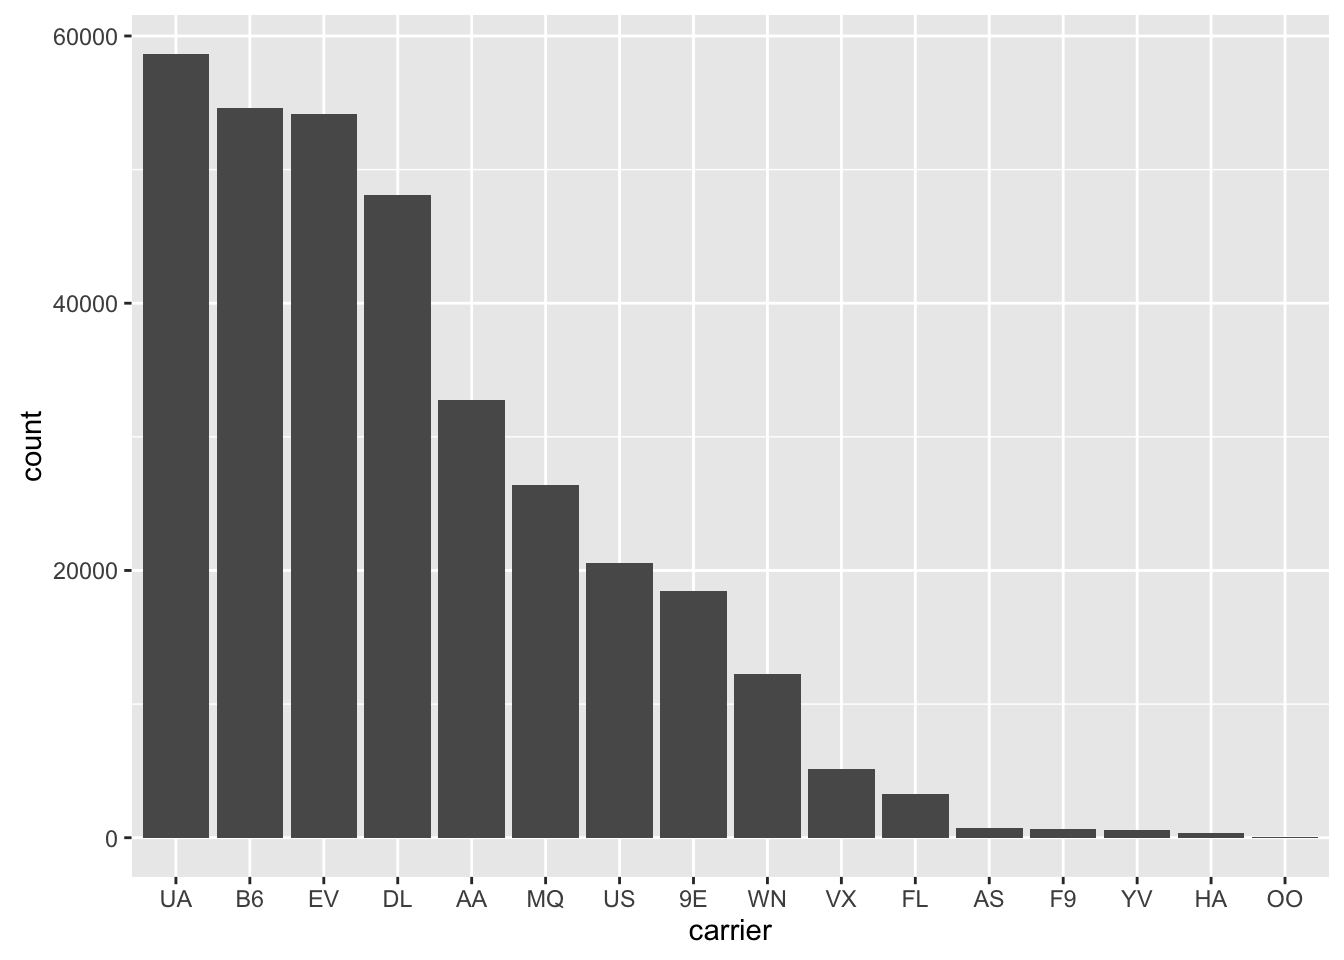
\includegraphics{ismay_kim_files/figure-latex/unnamed-chunk-38-1} \caption[Number of flights departing NYC in 2013 by airline - Descending numbers]{Number of flights departing NYC in 2013 by airline - Descending numbers}\label{fig:unnamed-chunk-38}
\end{figure}

\begin{Shaded}
\begin{Highlighting}[]
\CommentTok{#ggplot(data = carrier_counts, mapping = aes(x = carrier, y = n)) +}
\CommentTok{#  geom_bar(stat = "identity") + }
\CommentTok{#  scale_x_discrete(limits = carrier)}
\end{Highlighting}
\end{Shaded}

The last addition here specifies the values of the horizontal \texttt{x}
axis on a discrete scale to correspond to those given by the entries of
\texttt{sorted\_flights}.

** ** What are three specific questions that can be more easily answered
by looking at Figure 4.6 instead of Figure 4.5?

\begin{center}\rule{0.5\linewidth}{\linethickness}\end{center}

\begin{itemize}
\tightlist
\item
  Changing the labels of a plot (x-axis, y-axis)
\item
  Changing the theme for ggplots (\texttt{ggthemes} package too)
\item
  Adding \texttt{code\_folding} and \texttt{code\_download} to YAML
\end{itemize}

\bibliography{bib/packages.bib,bib/books.bib,bib/articles.bib}



\end{document}
